\documentclass[12 pt]{scrartcl}
\usepackage{setspace}
\usepackage{url}
\onehalfspacing
\usepackage{amsmath,amssymb,amsfonts,amsthm,mathtools}
\usepackage[english]{babel}
\usepackage[T1]{fontenc}
\usepackage[utf8x]{inputenc}
\usepackage{lmodern}
\usepackage{dsfont}
\usepackage{bbm}
\usepackage[round]{natbib}
\usepackage{color} 
\usepackage[defaultlines=2,all]{nowidow}
\usepackage{caption}
\usepackage[labelformat=simple]{subcaption}
\usepackage{makecell}
\renewcommand\thesubfigure{(\alph{subfigure})}

\setlength\parindent{0pt}
\setlength{\parskip}{6pt plus 1pt minus 1pt}

\newcommand{\red}{\textcolor{red}}


\begin{document}

\begin{titlepage}
  \centering
  {\scshape\LARGE TU Dortmund \par}
  \vspace{1cm}
  {\scshape\Large Case Studies \par}
  \vspace{2cm}
  {\huge\bfseries Project 2: BTA Deep Hole Drilling\par}
  \vspace{2cm}
  {\Large Lecturers:\\
    Dr.\ Uwe Ligges \\
    M.\ Sc.\ Marie Beisemann\\
    M.\ Sc.\ Leonie Schürmeyer \par}
  \vspace{1cm}
  {\Large Author: Tadeo Hepperle \par}
  \vspace{0.5 cm}
  {\Large Group number: 5\par}
  \vspace{0.5 cm}
  {\Large Group members: Lennard Heinrigs, Tadeo Hepperle, Joshua Oehmen, Vanlal Peka}
  \vfill
  {\large \today\par}
\end{titlepage}

\tableofcontents

\cleardoublepage

\section{Introduction}

% todo: explain what variables are present in the data

BTA deep hole drilling is a machining process that differs from traditional boring processes in some ways.
BTA stands for Boring and Trepanning Association and describes dilling processes in which the hole depth to diameter ratio is particularly large. BTA drilling machines can create holes of a diameter of 7mm up to 700 mm and can achieve a depth to diameter radius of up to 400:1
% https://unisig.com/information-and-resources/what-is-deep-hole-drilling/what-is-bta-drilling/
Because the holes are XXXX the boring head needs to be flexible


% explain what is chipping/zerspanung
% boring head usually self guiding. that is why it is a duynamic progress with distrubances
% https://en.wikipedia.org/wiki/Deep_hole_drilling

% How does BTA work?
% what materials are drilled in?? mainly metal???
% What is BTA used for?

% How does it differ from traditional drilling?

% We got measured data of XXX boring processes and want to see if we can predict chatter before onset.
% Goal: detect the onset of chattering before it happens.

\subsection{The Data}

To answer the question what causes chatter in BTA boring processes we take a look at data from 10 BTA drilling runs in this report.
As shown in Table \ref{tab:run_metadata}, each process has its own identifier (e.g. \emph{D4}), by which we refer to a process.
We refer to the processes \emph{D4}, \emph{D6} and \emph{D8} as \emph{D}-processes, while \emph{V2}, \emph{V6}, \emph{V10}, \emph{V17}, \emph{V20}, \emph{V24} and \emph{V25} are called \emph{V}-processes.
The \emph{D}-processes were recorded in 2002 and featured a damper installed 1240 mm away from clamping. In contrast to that the \emph{V}-processes were recorded in 2001 and did not use any damper in the BTA machine setup. It seems like the \emph{D}-processes do not show signs of chatter, while we can observe some form of chatter in all \emph{V}-processes.


\begin{table}[ht]
  \centering
  \captionabove{Drilling Processes and their Metadata}
  \label{tab:causes}
  \begin{tabular}{r|rrrr}
    \emph{identifier} & \emph{time} & \emph{cutting speed} & \emph{feed speed} & \emph{oil pressure} \\
    \hline
    \emph{D4}         & 3:54 min    & 111 m/min            & 0.231 mm/s        & unknown             \\
    \emph{D6}         & 4:28 min    & 120 m/min            & 0.185 mm/s        & unknown             \\
    \emph{D8}         & 4:27 min    & 90 m/min             & 0.250 mm/s        & unknown             \\
    \emph{V2}         & 4:51 min    & 120 m/min            & 0.185 mm/s        & unknown             \\
    \emph{V6}         & 4:25 min    & 111 m/min            & 0.231 mm/s        & 371 l/min           \\
    \emph{V10}        & 4:25 min    & 111 m/min            & 0.231 mm/s        & 229 l/min           \\
    \emph{V17}        & 4:44 min    & 120 m/min            & 0.185 mm/s        & 300 l/min           \\
    \emph{V20}        & 4:58 min    & 90 m/min             & 0.250 mm/s        & 300 l/min           \\
    \emph{V24}        & 4:29 min    & 120 m/min            & 0.185 mm/s        & 300 l/min           \\
    \emph{V25}        & 4:33 min    & 120 m/min            & 0.185 mm/s        & 300 l/min           \\
  \end{tabular}
\end{table}

There are a few parameters that are chosen in advance for each drilling process: \emph{cutting speed}, \emph{feed speed} and \emph{oil pressure}. Table \ref{tab:run_metadata} shows these parameters for the 10 processes.
The data for each of the 10 processes consists of a time series recording of several variables.
The time series data was recorded with a sampling rate of 20000Hz, so in each second of the boring process, 20000 observations of each of the measured variables have been recorded. That means there is no missing data and a consistent time gap of 0.05 ms between measurements. The time span of the drilling processes ranges from 3:54 min to 4:58 min.
The data was recorded utilizing the \emph{TEAC GX-1 Integrated Recorder} device, a machine developed by the \emph{TEAC} electronics company. The distribution of the device has been discontinued (SOURCE: https://daqlogsystems.co.uk/product/teac-gx-1/). The machine features a set of up to 8 input channels that can be fed with analog data.
Then, 16-bit A/D (analog to digital) converters convert the analog signal into a digital one, saving the measurement of each channel as a 16 bit signed integer.
The associated coefficients to convert the physical value to an integer value and vice versa need to be specified before the recording starts. They can be used to restore continous physical values from the 16-bit measurements. The data is stored in an \emph{interlaced} format. That means, for each point in time, the 16 bit value measured on each channel is appended to a file. So if we split the resulting file into chunks of $2*\emph{NUMBER\_OF\_CHANNELS}$ bytes, each of these chunks represents one point in time.

The following variables were measured for all 10 processes:
\begin{itemize}
  \item \emph{acoustic} - the audio signal in Pa (Pascal), noise and sound during the drilling process
  \item \emph{moment} - the torsianal moment in Nm (Newtonmeter), also known as drilling torque. Measured at the drilling bar above the bore hole of the BTA drilling machine. It is created by forces of chipping, friction and deformation at the guide rails.
  \item \emph{sync signal} - an electric signal that is triggered by the drilling head having a certain axial rotation. It flows once per revolution of the drilling head for a brief moment.
  \item \emph{oil acceleration} - the acceleration of the drilling oil supply in $m/s^2$
  \item \emph{force} - the force in feed direction in N (Newton). It is related to the \emph{feed speed} but also to the resistance (hardness) the work piece material has against being drilled
\end{itemize}

Besides that, the 7 \emph{V}-processes feature 2 additional variables for the acceleration of the drilling head: \emph{lateral acceleration} and \emph{frontal acceleration} (acceleration in frontal direction) each measured in $m/s^2$.
The 3 \emph{D}-processes also contain the \emph{bending moment} in Nm as a variable. They also contain measurements on a variable called "bohrst", but it remains unclear to us what this variable stands for. It is measured in $m/s^2$ but more we do not know, hence we do not further discuss it in this report.

\subsubsection{Labels} \label{labels}

The data we received is unlabeled. That means we just have the time series of the predictor variables, but do not know in what time regions chatter appears. The only thing we could do is listen to the audio signal. Because chatter can be heard as a resonating frequency, we were able to manually label each process and divide it into different time segments:

\begin{itemize}
  \item \emph{start} - before the boring head made contact to the material.
  \item \emph{no chatter} - normal drilling, no audible chatter.
  \item \emph{chatter} - audible chatter, recognizable as constistent high tones in the audio.
  \item \emph{low chatter} - audible chatter, but rather low tones. Often present after some time of high tones chatter.
  \item \emph{end} - after the boring head is done with drilling and no pressure is asserted on the material anymore
\end{itemize}

The time segments appear in each process in this order, sometimes skipping the \emph{chatter} and \emph{low chatter} stages.
The main focus of this report is to detect the change from \emph{no chatter} to \emph{chatter} with some procedure that would work online only with data from \textbf{before} the \emph{chatter} stage is entered.



\subsection{Prior Research}

% What attempts have been made in research to model these time series??

% just audio does not work well (WHO said tha XXXXXX)
% - neural networks
% - area under ACF and KOlgomerov smirnov
% - frequency based????

% how did WE do it?? What methods did we use???

% what variables are important? What does prior research indicate?

\section{Methods}

This chapter briefly explains the statistical methods used. to apply them we use Python \citep{python} as statistical software. The Python packages numpy \citep{numpy}, pandas \citep{pandas}, matplotlib \citep{matplotlib} and mlxtend \citep{mlxtend} have been used. In addition we developed a custom python package called \emph{gx1convert} \citep{gx1convert} that was used to read in the data produced by the GX-1 device.

% For reading the data, I developed a package that can read any gx1 time series. Availbale here: XXXXX
% python was used for all data analysis. These packages:  TAKE FROM REPORT 1

\subsection{Power Spectrum}

% Fourrier transform????


\subsection{Covariance and Correlation}

Given a set of $n$ datapoints each consisting of a value on two metric variables X and Y, their covariance $s_{XY}$ can be computed as the product of the difference to the respective variable mean summed up for all datapoints and divided by $n$.

\[ s_{XY} = \frac{1}{n} \cdot  \sum_{i=1}^{n}{(x_i - \overline{x}) \cdot (y_i - \overline{y})}\]

It is a measure of how much the variables vary together linearly in the same direction.
Because the covariance greatly depends on the units of measurement, it can be standardized to a range between $-1$ and $+1$ by dividing it by the standard deviations of both variables.

\[ r_{XY} =  \frac{s_{XY}}{s_X \cdot s_Y} \]

The result $r_{XY}$ is known as Pearson's r or Pearson product-moment correlation coefficient. Note that $r_{XY}$ is symmetrical, so $r_{XY} = r_{YX}$ and in case that either $s_X$ or $s_Y$ is zero it is not defined. It is a standardized measure of linear correlation between two metric variables \citep[p.~538]{eid2017statistik}. A correlation of $r_{XY} = 1$ means perfect correlation.


\subsection{Auto-Correlation Function (ACF)}

The auto-correlation function (ACF) shows how much a time series is correlated with a lagged version of itself. For a Time series $X_t$ consisting of $n$ data points $x_1, ..., x_n$ the ACF is defined as a function $\rho(k)$ that maps an integer $k$ to the correlation of $X_t$ with $X_{t+1}$ (SOURCE XXX TIME SERIES BOOK PAGE 4):

\[ \rho(k) = Corr(X_t, X_{t+1}) \]

In this equation, $k$ represents a lag value. In time series analysis we call a "lag", a shift of the time series along the temporal direction. The correlation is calculated over all possible values of $t$ where $1 \le t \le n - k$.For example for values $t = 3$ and $k = 2$, the variable $X_t$ would refer to the data point $x_3$ and $X_t$ would be $x_5$. From the equation follows that $\rho(0)$ is always 1, because $\rho(0) = Corr(X_t, X_t) = 1$. Because the ACF for higher lag values has less data point pairs available for correlation calculation, one should only calculate the ACF for lag values much less than the length of the time series itself.
Interpreting the ACF only makes sense if the underlying process is (weakly) stationary (SOURCE XXX TIME SERIES PAGE 4). This should be given if we look at regions of a drilling process where mean and variance do not change too much. Periodicities in a time series also show as periodic patterns in the ACF.

% relationship between acf AND SFT

\subsubsection{Absolute Area under the ACF ($A_{ACF}$)}

XXX mention, that they used the ACF in a strategy to detect chatter in BTA drilling processes. Because the ACF carries information about periodic correlations in the time series, it should contain information of chatter. They selected a range of L lags $k \in \{0, ..., L\}$ and calculated the ACF $\rho(k)$ for each lag value. Then they summed up the absolute value.

\[ A_{ACF} = \sum^{L}_{h=0}{|p(h)|} \]

XXX chose a value of L=30 in their approach and calculated this $A_{ACF}$ value for small chunks of time cut out of the original time series.
If there are strong resonating frequencies in the data, the $A_{ACF}$ value is expected to be higher.

\section{Data Analysis}

We manually labeled each process as into segments as described in section \ref{labels}. Table \ref{tab:segmenttime} shows the time regions we determined for each segment in seconds:

\begin{table}[ht]
  \centering
  \captionabove{Time Segments of each Drilling Process}
  \label{tab:segmenttime}
  \begin{tabular}{r|rrrrr}
               & \emph{start} & \emph{no chatter} & \emph{chatter} & \emph{low chatter} & \emph{end} \\
    \hline
    \emph{D4}  & 0 - 3        & 3  - 222          & /              & /                  & 222 - 234  \\
    \emph{D6}  & 0 - 2        & 2  - 254          & /              & /                  & 254 - 268  \\
    \emph{D8}  & 0 - 4        & 4  - 254          & /              & /                  & 254 - 267  \\
    \emph{V2}  & 0 - 10       & 10 - 200          & 200 - 264      & /                  & 264 - 291  \\
    \emph{V6}  & 0 - 31       & 31 - 47           & 47  - 136      & 136 - 253          & 253 - 265  \\
    \emph{V10} & 0 - 31       & 31 - 47           & 47  - 91       & 91  - 252          & 252 - 264  \\
    \emph{V17} & 0 - 16       & 16 - 35           & 35  - 45       & 45  - 270          & 270 - 284  \\
    \emph{V20} & 0 - 33       & 33 - 52           & 52  - 136      & 136 - 287          & 287 - 298  \\
    \emph{V24} & 0 - 3        & 3  - 22           & 22  - 64       & 64  - 258          & 258 - 269  \\
    \emph{V25} & 0 - 5        & 5  - 118          & 118 - 260      & /                  & 260 - 272  \\
  \end{tabular}
\end{table}

The end point of the \emph{start} segment and the start point of the \emph{end} segment were best identified by looking at the \emph{force} time series for each process. The force quickly increases in abolute value when the BTA drilling head makes contact with the workpiece and falls when it is released, as visible in Figure \ref{fig:all-force}.
We also plotted the time series for \emph{moment}, \emph{sync signal}, \emph{oil acceleration} and \emph{acoustic} for all processes together with the time segements. They can be found in Figure \ref{all-moment} to Figure \ref{all-acoustic} in the Appendix. For the \emph{V}-processes Figure \ref{fig:all-frontal} and Figure \ref{fig:all-lateral} show the frontal and lateral acceleration respectively. The reason for plotting all of these variables in conjuction with the time segments is, that it helps us identify which variables show a visible difference between the chatter and non-chatter regions. It looks like only the \emph{acoustic} signal and the \emph{moment} and \emph{oil acceleration} show visible differences.

\subsection{Frequencies and ACF}

We now want to take a look at the frequency space. Figure \ref{fig:v2-spec} shows the spectrogram for the \emph{V2}-Process.
The area between the blue and purple line is the \emph{non-chatter} segment, while the area between the purple and blue line marks the \emph{chatter} segment. We can see that \emph{force}, \emph{moment}, \emph{acoustic} and \emph{oil acceleration} show changes in their pattern as soon as the chatter appears. But there does not seem to be a pattern forming, before the chatter starts.

\begin{figure}[p]
  \makebox[\linewidth]{
    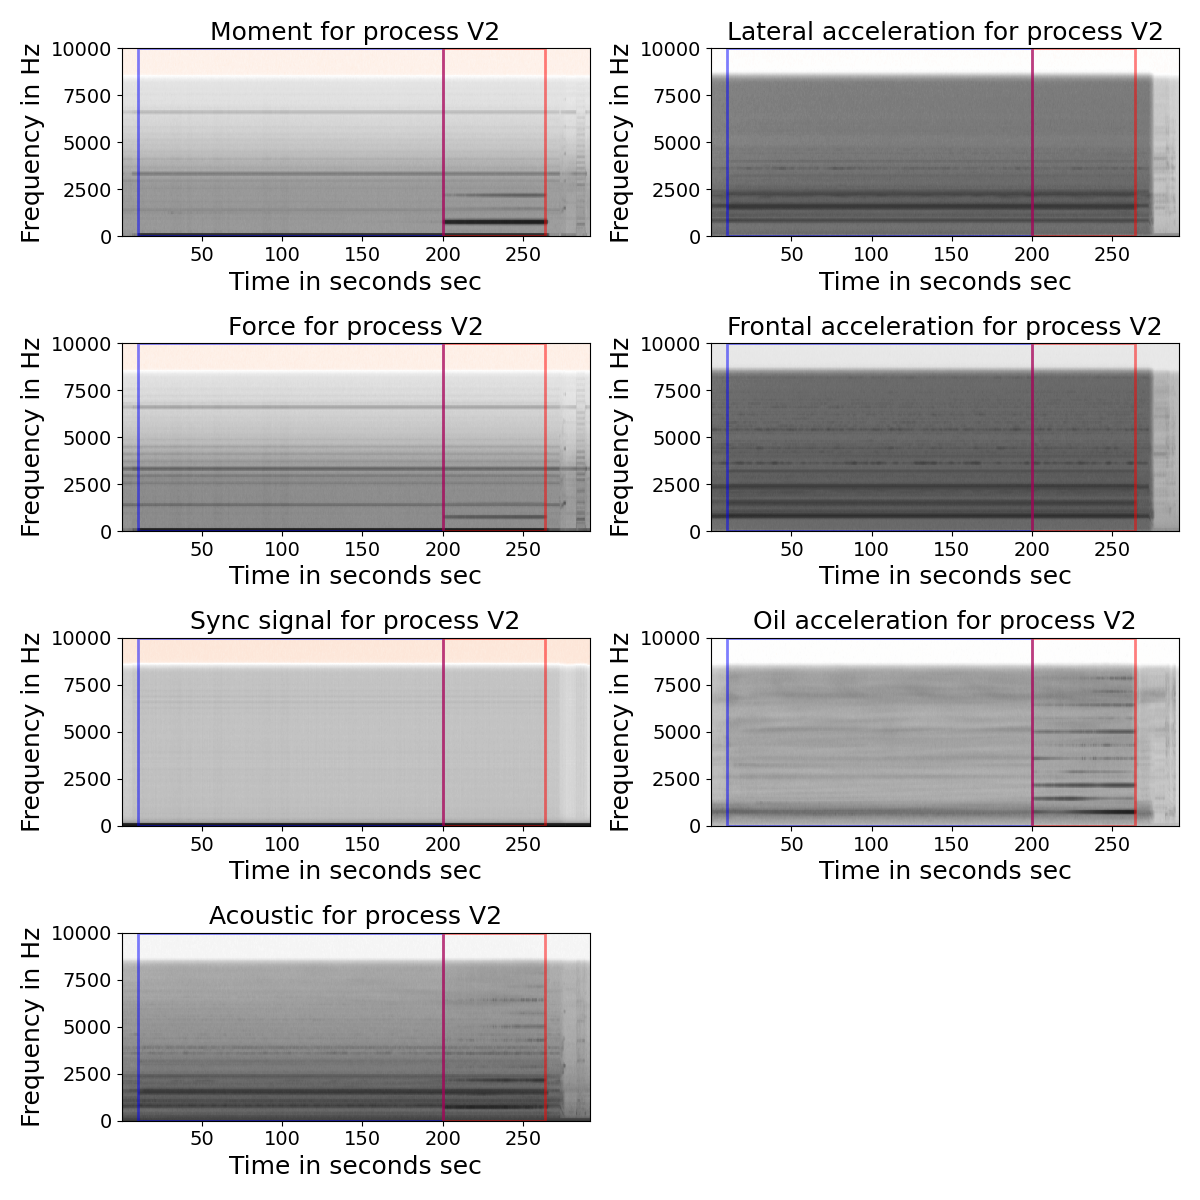
\includegraphics[width=0.9\linewidth]{../plots/v2-spec.png}
  }
  \caption{Spectrogram for the \emph{V2}-Process}
  \label{fig:v2-spec}
\end{figure}

If we assume that chatter is in general associated with the workpiece resonating certain frequencies, it is not surprising to see patterns to be more pronounced in the \emph{chatter} segment. Using all data points from the \emph{chatter} and \emph{non-chatter} regions respectively we calculate the ACF up to lag 100 for each variable of the \emph{V2}-process. We are looking for a variable where the ACF differs a lot between \emph{chatter} and \emph{non-chatter} regions. This would allow us then to witness how the ACF changes from its \emph{non-chatter} form to the \emph{chatter} constellation and shut down the machine before we fully reach the \emph{chatter phase}.

\begin{figure}[p]
  \makebox[\linewidth]{
    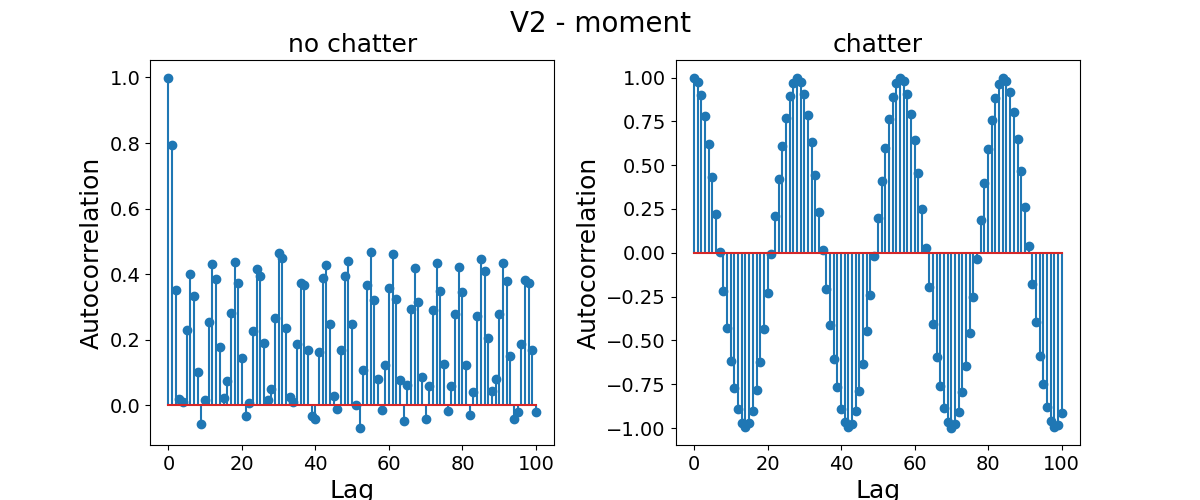
\includegraphics[width=0.9\linewidth]{../plots/v2-moment-acfs.png}
  }
  \caption{ACF for the \emph{moment} variable of the \emph{V2} process in two regions}
  \label{fig:v2-moment-acfs}
\end{figure}


\begin{figure}[p]
  \makebox[\linewidth]{
    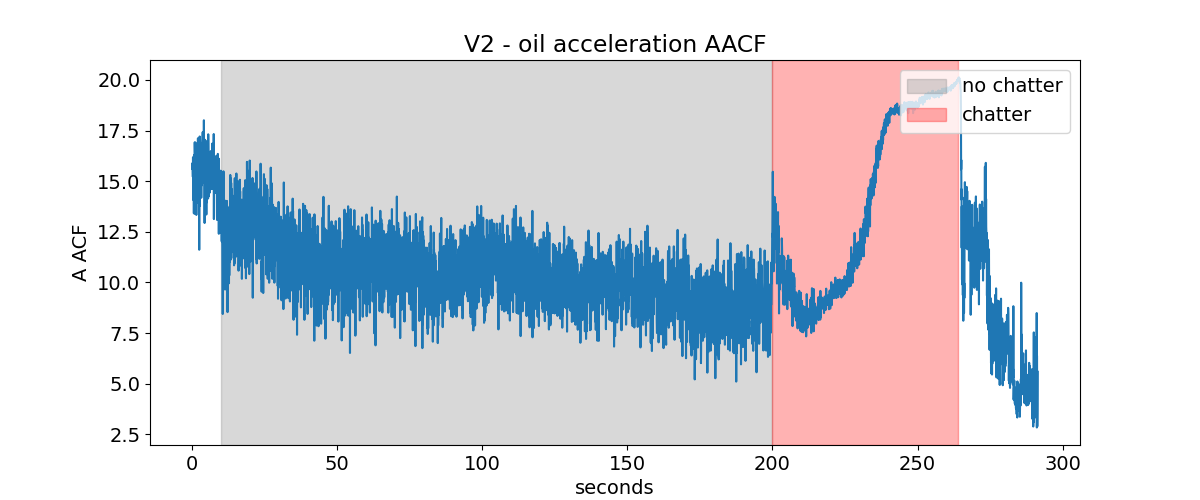
\includegraphics[width=0.9\linewidth]{../plots/v2-oil acceleration-acfs.png}
  }
  \caption{ACF for the \emph{oil acceleration} variable of the \emph{V2} process in two regions}
  \label{fig:v2-oil-acfs}
\end{figure}


Figure \ref{fig:v2-moment-acfs} and Figure \ref{fig:v2-oil-acfs} show a very regular periodic pattern in the ACF for the \emph{chatter} phase for the variables \emph{moment} and \emph{oil acceleration}. The wavelength seems to be around 30 lags. Since $20000/30 \approx 667$ this lag constellation would suggest a dominant frequency of around 667 Hz. This is also visible as a thick black horizontal line in the \emph{chatter} region of the top left spectrogram of Figure \ref{fig:v2-spec} (\emph{moment} variable) at around this frequency.
In the \emph{non-chatter} regions the behavior of the ACF differs between the two variables though: \emph{oil acceleration} shows some slowly decaying pattern, where after 100 lags almost no correlation is left, while we can observe some high frequent oscillations in the ACF of \emph{moment}.

\begin{figure}[p]
  \makebox[\linewidth]{
    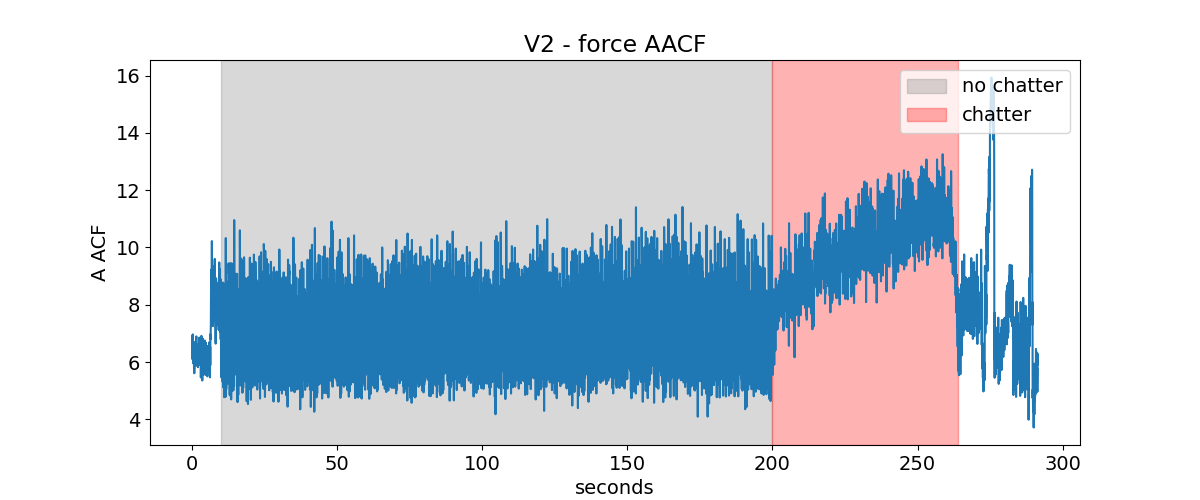
\includegraphics[width=0.9\linewidth]{../plots/v2-force-acfs.png}
  }
  \caption{ACF for the \emph{force} variable of the \emph{V2} process in two regions}
  \label{fig:v2-force-acfs}
\end{figure}


\begin{figure}[p]
  \makebox[\linewidth]{
    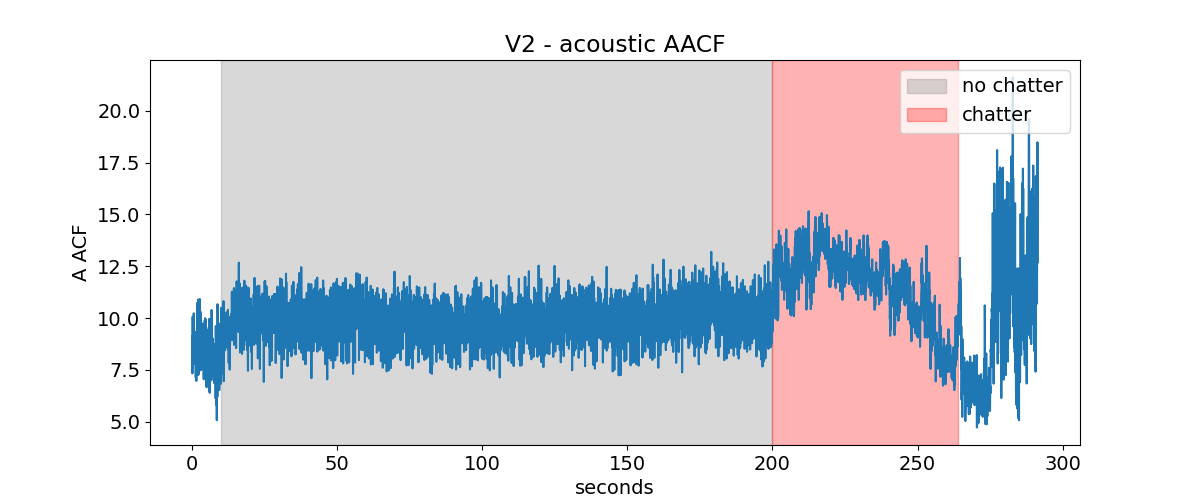
\includegraphics[width=0.9\linewidth]{../plots/v2-acoustic-acfs.png}
  }
  \caption{ACF for the \emph{acoustic} variable of the \emph{V2} process in two regions}
  \label{fig:v2-acoustic-acfs}
\end{figure}

Figure \ref{fig:v2-acoustic-acfs} and  Figure \ref{fig:v2-force-acfs} shows that the ACFs of the \emph{acoustic} and the \emph{force} channel show similar behavior, but the ACF in the \emph{chatter} region is not as regular as in the \emph{moment} channel. The \emph{sync signal},
\emph{lateral acceleration} and \emph{frontal acceleration} variables are probably not very useful to detect chatter: The ACFs for \emph{chatter} vs. \emph{non chatter} segments in Figure \ref{fig:v2-sync-acfs}, \ref{fig:v2-lateral-acfs} and \ref{fig:v2-frontal-acfs} do not really differ.


\begin{figure}[p]
  \makebox[\linewidth]{
    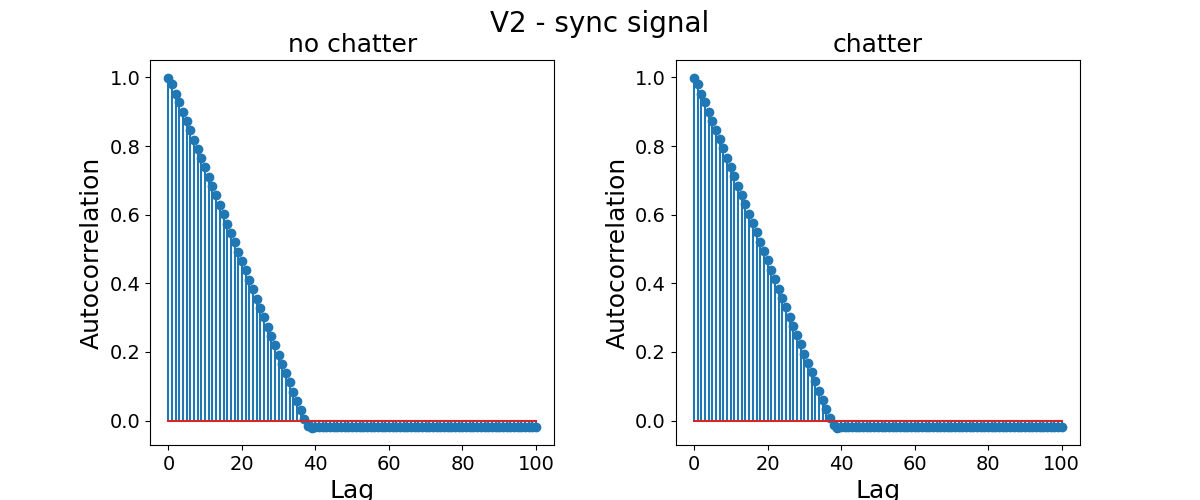
\includegraphics[width=0.9\linewidth]{../plots/v2-sync signal-acfs.png}
  }
  \caption{ACF for the \emph{sync signal} variable of the \emph{V2} process in two regions}
  \label{fig:v2-sync-acfs}
\end{figure}


\begin{figure}[p]
  \makebox[\linewidth]{
    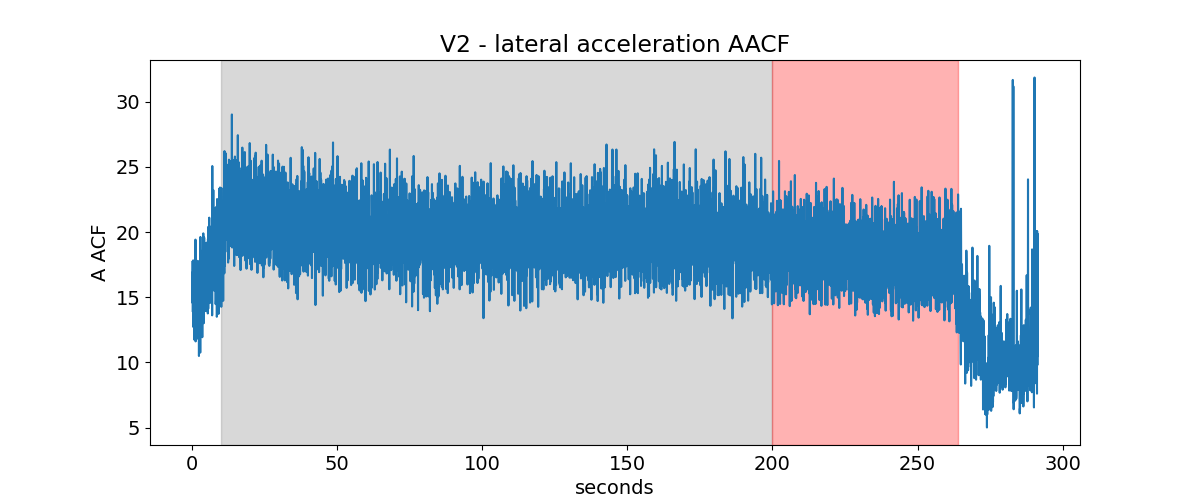
\includegraphics[width=0.9\linewidth]{../plots/v2-lateral acceleration-acfs.png}
  }
  \caption{ACF for the \emph{lateral acceleration} variable of the \emph{V2} process in two regions}
  \label{fig:v2-lateral-acfs}
\end{figure}


\begin{figure}[p]
  \makebox[\linewidth]{
    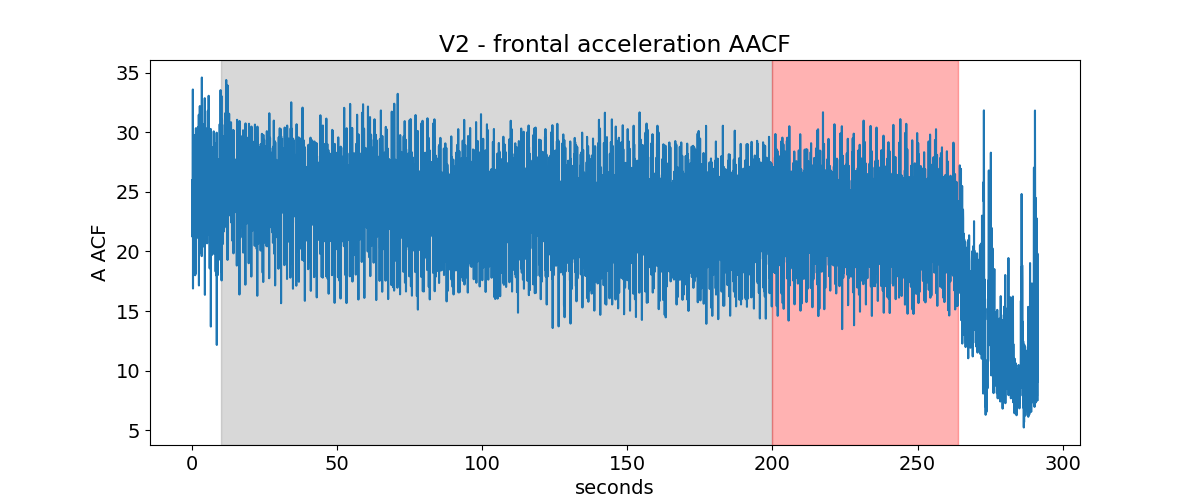
\includegraphics[width=0.9\linewidth]{../plots/v2-frontal acceleration-acfs.png}
  }
  \caption{ACF for the \emph{frontal acceleration} variable of the \emph{V2} process in two regions}
  \label{fig:v2-frontal-acfs}
\end{figure}

\subsection{Detect chatter with $A_{ACF}$}

We now split the time series into chunks with a width of 1000 data points. That is the equivalent of 50ms for each chunk. For each of these chunks we calculate the ACF up to lag 100.
Using a similar approach as XXX(Statistics and Time Series Analyses of...)XXX we reduce these 101 coefficients down to an $A_{ACF}$ value that represents the absolute area under the autocorrelation function $A_{ACF} = \sum^{L}_{h=0}{|p(h)|}$.
Here $p(h)$ is the autocorrelation at lag $h$ calculated on the respective 1000-point chunk. Using this approach the \emph{non-chatter} segments had between 320 and 3800 chunks and the \emph{chatter} segments we composed of 200 to 2840 chunks each. Table \ref{tab:aacfstats} shows for each of the processes the average $A_{ACF}$ values in the \emph{chatter} and \emph{non-chatter} regions.

\begin{table}[ht]
  \centering
  \captionabove{$A_{ACF}$ from ACF up to lag 100 for \emph{moment} in \emph{non-chatter} and \emph{chatter} segments. N = \emph{non-chatter}, C = \emph{chatter}}
  \label{tab:aacfstats}
  \begin{tabular}{l|rr|rr|rr|rr}
    process & \multicolumn{2}{c|}{\emph{mean}} & \multicolumn{2}{c|}{\emph{std}} & \multicolumn{2}{c|}{\emph{min}} & \multicolumn{2}{c|}{\emph{max}}                                \\
            & N                                & C                               & N                               & C                               & N    & C     & N     & C     \\
    \hline
    D4      & 12.85                            &                                 & 2.54                            &                                 & 7.59 &       & 44.61 &       \\
    D6      & 13.21                            &                                 & 4.48                            &                                 & 4.59 &       & 41.27 &       \\
    D8      & 14.45                            &                                 & 3.60                            &                                 & 5.94 &       & 39.38 &       \\
    V2      & 19.56                            & 61.54                           & 8.43                            & 0.06                            & 5.79 & 61.15 & 60.16 & 61.73 \\
    V6      & 11.49                            & 60.48                           & 7.04                            & 1.80                            & 5.21 & 37.51 & 44.64 & 61.04 \\
    V10     & 10.88                            & 60.75                           & 5.43                            & 1.16                            & 5.37 & 33.88 & 36.69 & 61.02 \\
    V17     & 16.89                            & 59.57                           & 11.19                           & 3.81                            & 4.99 & 35.90 & 61.04 & 61.29 \\
    V20     & 13.13                            & 58.62                           & 7.54                            & 3.17                            & 5.42 & 32.63 & 50.40 & 61.95 \\
    V24     & 12.23                            & 60.54                           & 8.81                            & 1.81                            & 5.50 & 39.58 & 60.90 & 62.93 \\
    V25     & 21.35                            & 61.09                           & 14.56                           & 0.95                            & 6.02 & 42.54 & 60.92 & 61.68 \\
  \end{tabular}
\end{table}

We can see that all time series show an average $A_{ACF}$ value of around 10 - 21 in the non-chatter regions. Those processes that show chatter have average $A_{ACF}$ values of 58.62 to 61.54 in the chatter regions. That is a large difference. One way to interpret the $A_{ACF}$ values is, as a measure of how much any measured value can be predicted by the preceeding 100 values. This however is not very close to the truth, because it does not account for shared predictive variance between different lag values. What Table \ref{tab:aacfstats} also shows it, that for all \emph{V}-processes the variance of the $A_{ACF}$ values is lower in the \emph{chatter} segments than in the \emph{non-chatter} segments. This is not surprising, because chatter is all about similar vibrations occuring for some time.
But it is also true, that some chunks in the \emph{non-chatter} segments have higher $A_{ACF}$ values that some chunks of the \emph{chatter} region of the same process, as the \emph{min} and \emph{max} columns in the table show. So to develop a policy that allows us to detect chatter based on the $A_{ACF}$ value we need to take a closer look at some graphs.

\begin{figure}[p]
  \makebox[\linewidth]{
    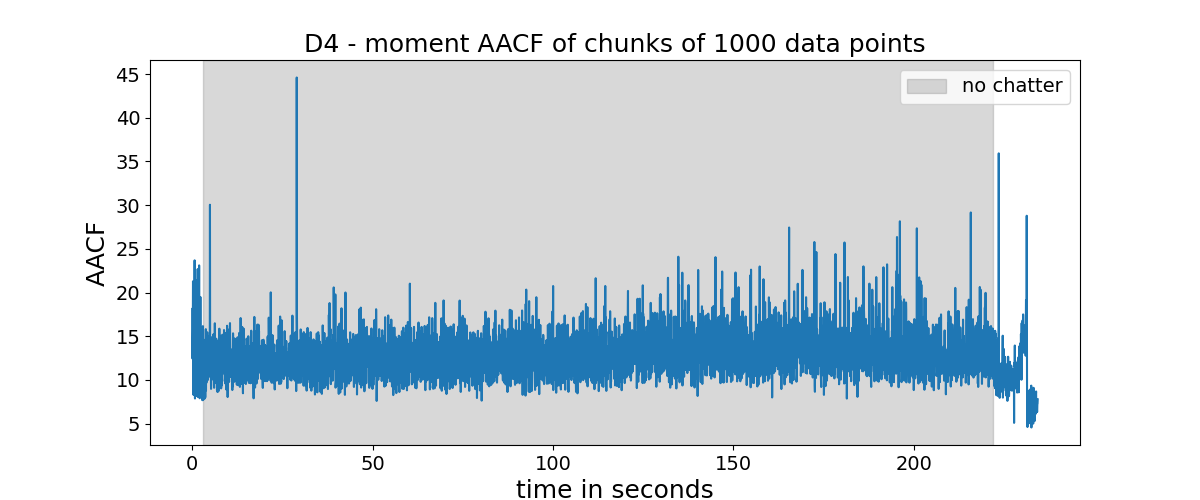
\includegraphics[width=0.9\linewidth]{../plots/d4-moment-aacf.png}
  }
  \caption{\emph{D4} process: $A_{ACF}$ for \emph{moment} variable}
  \label{fig:d4-moment-aacf}
\end{figure}


\begin{figure}[p]
  \makebox[\linewidth]{
    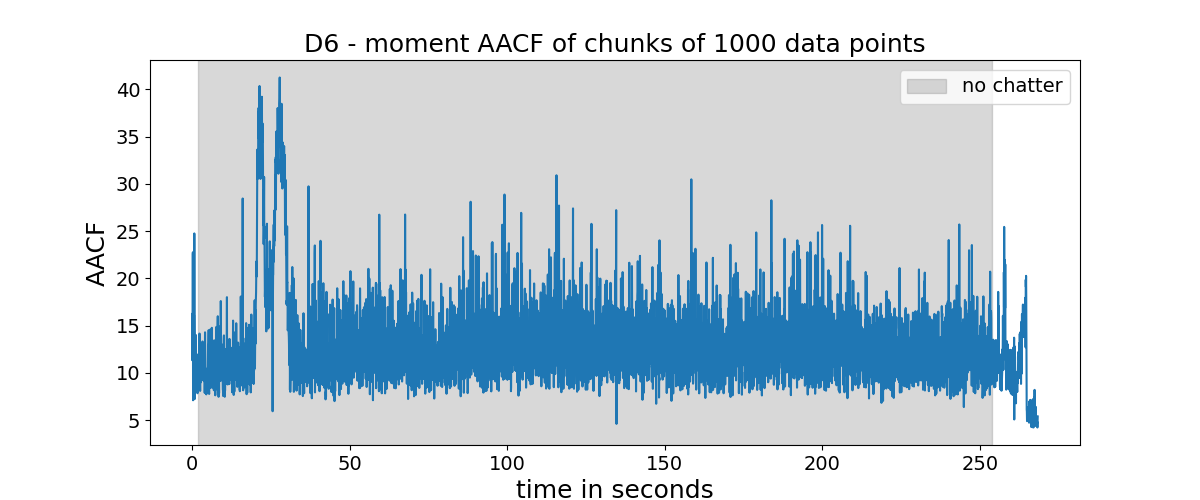
\includegraphics[width=0.9\linewidth]{../plots/d6-moment-aacf.png}
  }
  \caption{\emph{D6} process: $A_{ACF}$ for \emph{moment} variable}
  \label{fig:d6-moment-aacf}
\end{figure}


\begin{figure}[p]
  \makebox[\linewidth]{
    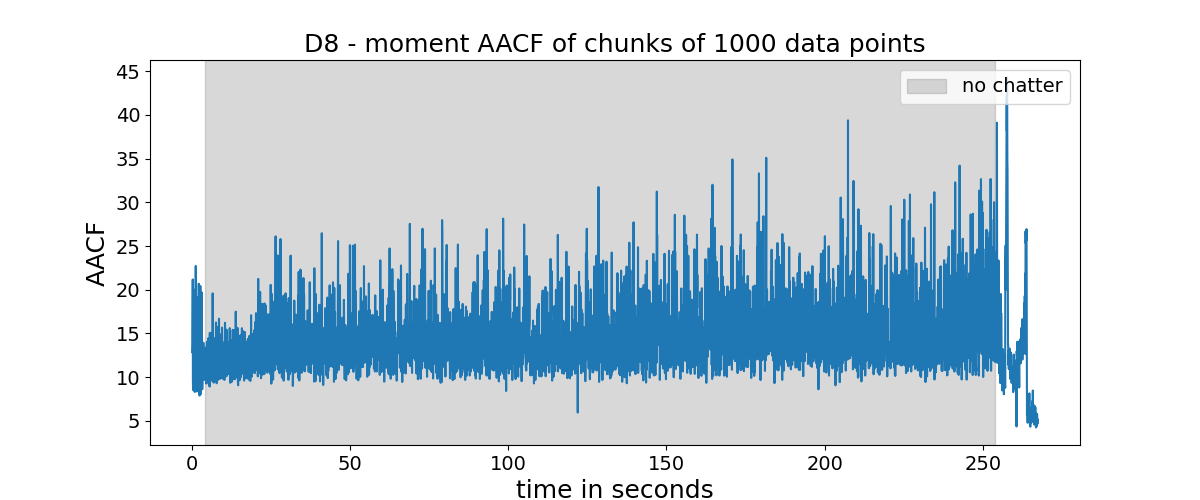
\includegraphics[width=0.9\linewidth]{../plots/d8-moment-aacf.png}
  }
  \caption{\emph{D8} process: $A_{ACF}$ for \emph{moment} variable}
  \label{fig:d8-moment-aacf}
\end{figure}

Firstly plotting the $A_{ACF}$ value of the \emph{moment} variable for each chunk of the \emph{D}-processes shows us that the $A_{ACF}$ varies a bit but never reaches values greater than 45 (See Figure \ref{fig:d4-moment-aacf}, \ref{fig:d6-moment-aacf} and \ref{fig:d8-moment-aacf}).



\begin{figure}[p]
  \makebox[\linewidth]{
    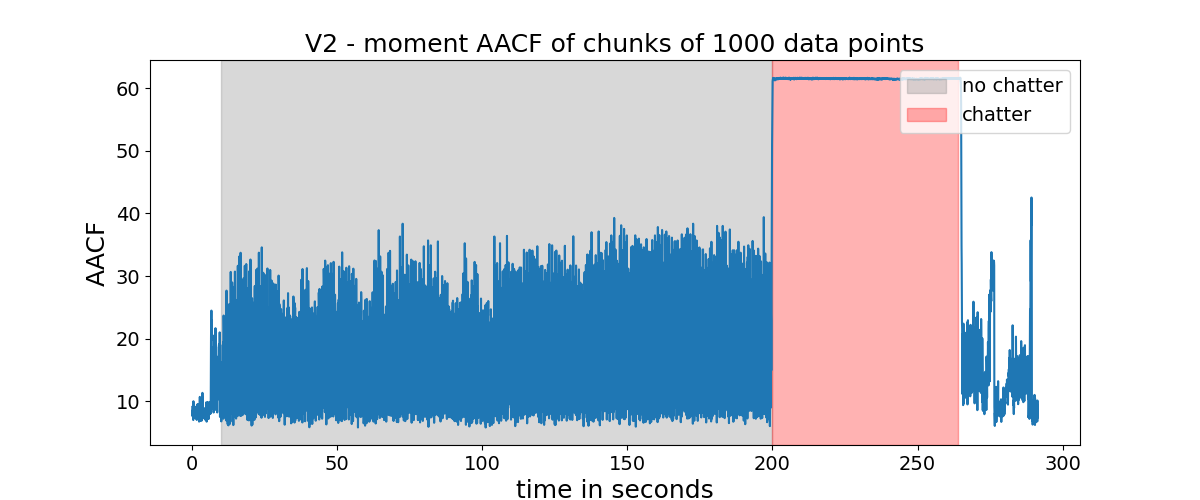
\includegraphics[width=0.9\linewidth]{../plots/v2-moment-aacf.png}
  }
  \caption{\emph{V2} process: $A_{ACF}$ for \emph{moment} variable}
  \label{fig:v2-moment-aacf}
\end{figure}



\begin{figure}[p]
  \makebox[\linewidth]{
    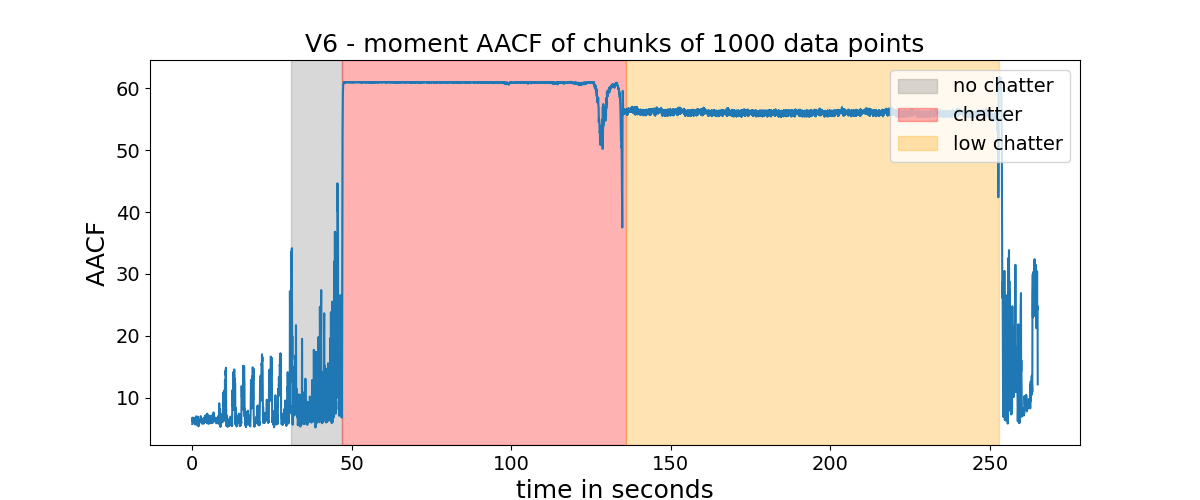
\includegraphics[width=0.9\linewidth]{../plots/v6-moment-aacf.png}
  }
  \caption{\emph{V6} process: $A_{ACF}$ for \emph{moment} variable}
  \label{fig:v6-moment-aacf}
\end{figure}



\begin{figure}[p]
  \makebox[\linewidth]{
    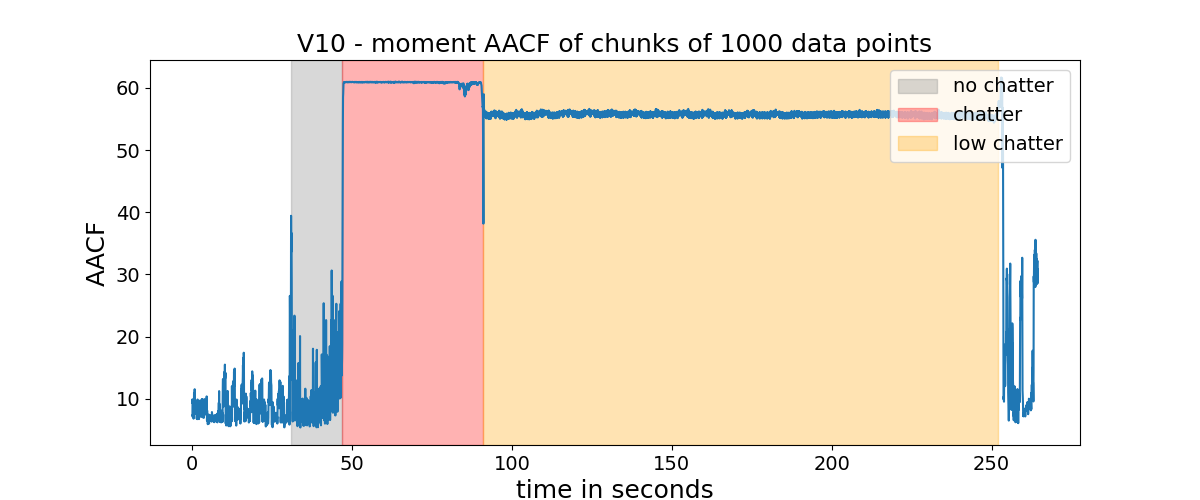
\includegraphics[width=0.9\linewidth]{../plots/v10-moment-aacf.png}
  }
  \caption{\emph{V10} process: $A_{ACF}$ for \emph{moment} variable}
  \label{fig:v10-moment-aacf}
\end{figure}



\begin{figure}[p]
  \makebox[\linewidth]{
    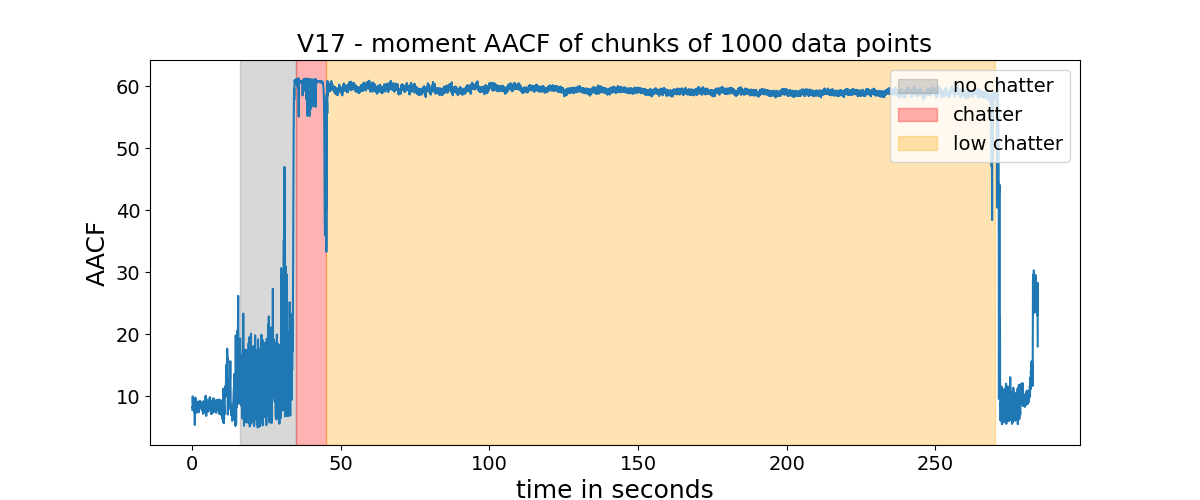
\includegraphics[width=0.9\linewidth]{../plots/v17-moment-aacf.png}
  }
  \caption{\emph{V17} process: $A_{ACF}$ for \emph{moment} variable}
  \label{fig:v17-moment-aacf}
\end{figure}


\begin{figure}[p]
  \makebox[\linewidth]{
    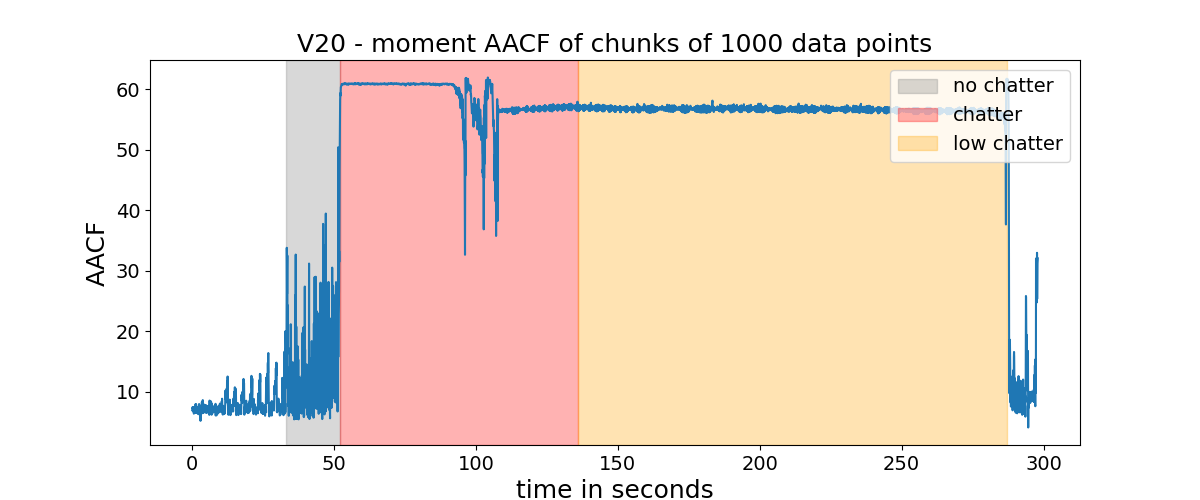
\includegraphics[width=0.9\linewidth]{../plots/v20-moment-aacf.png}
  }
  \caption{\emph{V20} process: $A_{ACF}$ for \emph{moment} variable}
  \label{fig:v20-moment-aacf}
\end{figure}


\begin{figure}[p]
  \makebox[\linewidth]{
    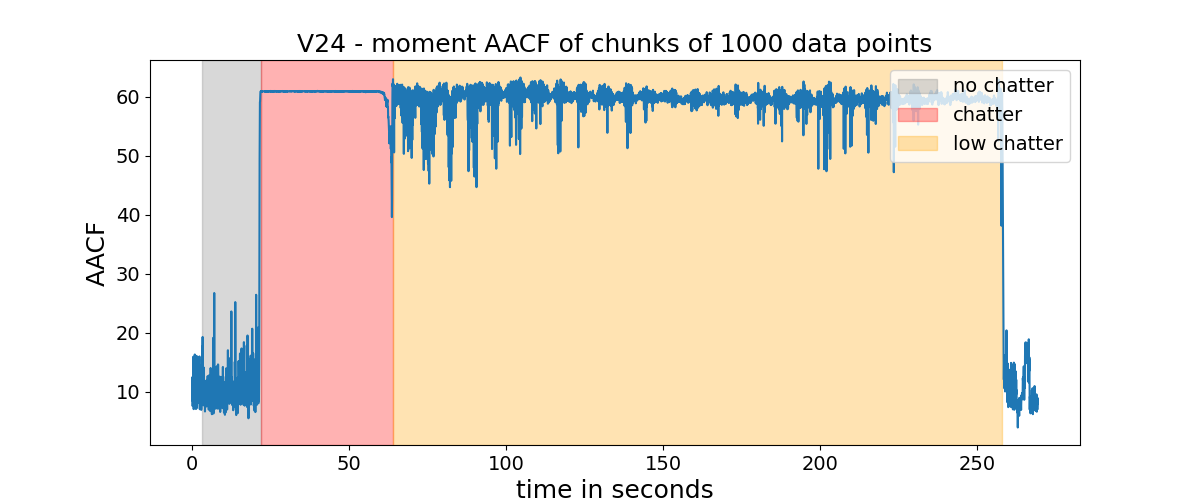
\includegraphics[width=0.9\linewidth]{../plots/v24-moment-aacf.png}
  }
  \caption{\emph{V24} process: $A_{ACF}$ for \emph{moment} variable}
  \label{fig:v24-moment-aacf}
\end{figure}


\begin{figure}[p]
  \makebox[\linewidth]{
    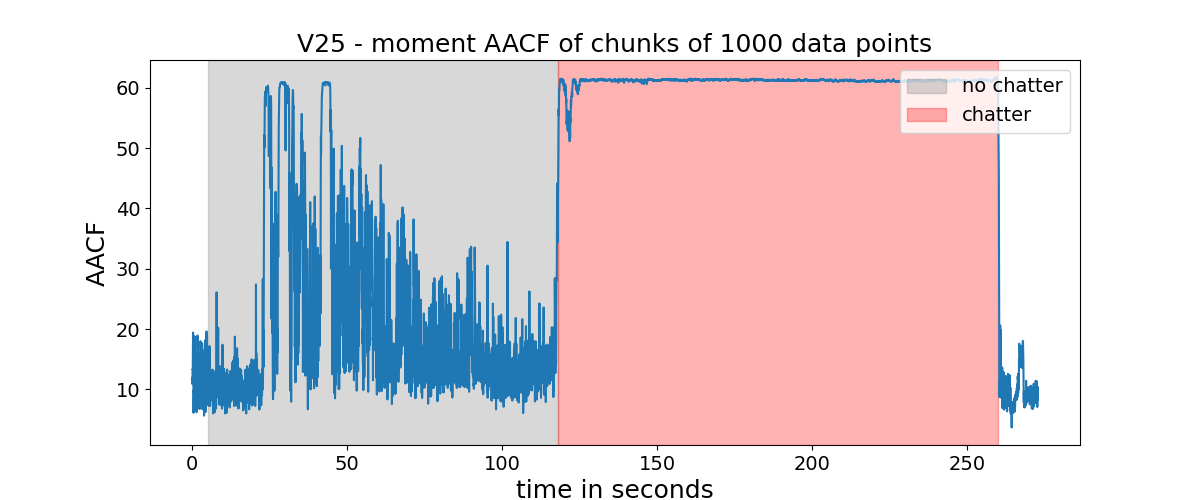
\includegraphics[width=0.9\linewidth]{../plots/v25-moment-aacf.png}
  }
  \caption{\emph{V25} process: $A_{ACF}$ for \emph{moment} variable}
  \label{fig:v25-moment-aacf}
\end{figure}

For all of the \emph{V}-processes we can see a similar behavior of the $A_{ACF}$ when entering the \emph{chatter} region: The $A_{ACF}$ shoots up to a value around 60 and then stays relatively constant for almost the entire \emph{chatter} period. During the \emph{low chatter} segment, that often follows, the $A_{ACF}$ is a bit lower and not so low in variance, but still higher than when no chatter occurs. If we were to stop the machine as soon as the $A_{ACF}$ surpasses a value of 50, we are right in the beginning or the chatter in most cases. There is only one processe, \emph{V25} where $A_{ACF}$ values occur during the normal boring process without being closely followed by chatter. This can be observed in Figure \ref{fig:v25-moment-aacf}.
We now want to determine if the high $A_{ACF}$ values have predictive power that make a prediction leading up to the \emph{chatter} region possible. It could also be that they only occur once we are already inside the chatter region, which would mean we would have to accept a little bit of chatter before the machine can be stopped.
Going by the cutoff rule of $A_{ACF} = 50$ we can now determine for each \emph{V}-process at which point in time the threshold is surpassed for the first time.
Table \ref{tab:pointdiff} shows when the threshold of $A_{ACF} = 50$ is surpassed for the first time for each of the 7 \emph{V}-processes. Negative values in the second column indicate that the threshold was reaches before being in the \emph{chatter} segment.

\begin{table}[ht]
  \centering
  \captionabove{Time difference between the first point where $A_{ACF} > 50$ and start of \emph{chatter} segment.}
  \label{tab:pointdiff}
  \begin{tabular}{l|rr}
    \\
    process & time     & difference \\
    \hline
    V2      & 199.85 s & -0.15 s    \\
    V6      & 47.15 s  & 0.15 s     \\
    V10     & 47.15 s  & 0.15 s     \\
    V17     & 34.15 s  & -0.85 s    \\
    V20     & 51.45 s  & -0.55 s    \\
    V24     & 21.55 s  & -0.45 s    \\
    V25     & 23.25 s  & -94.75 s   \\
  \end{tabular}
\end{table}

Out of the 7 processes, 6 were able to locate the start of chatter within a tolerance window of 1 seconds. Only process \emph{V25} gave a very early alarm (See \ref{fig:v25-moment-aacf}).
It is important to note that the exact value and sign of the difference should not be overinterpreted, as long as it is in the subsecond range. This is because the beginning and end time points of \emph{chatter} and \emph{non-chatter} regions were determined manually by listening to the audio signal. It is hard to tell the \emph{exact} point in time when chatter starts.
We do not want to investigate the \emph{low chatter} regions that were determined by the same method. The objective of this report is, to find out how to predict the start of the chatter. Splitting chatter into \emph{chatter} and \emph{low chatter} was only done to have more uniform time segments to analyze.

\section{Summary and Discussion}

% this is too little data to do much. Also variables different between data.

\newpage
\addcontentsline{toc}{section}{Bibliography}
\renewcommand\refname{Bibliography}
\bibliographystyle{plainnat}
\bibliography{references}
\newpage
\appendix
\addsec{Appendix}
\subsection*{A \ Additional figures}




\begin{figure}[p]
  \vspace*{-1cm}
  \makebox[\linewidth]{
    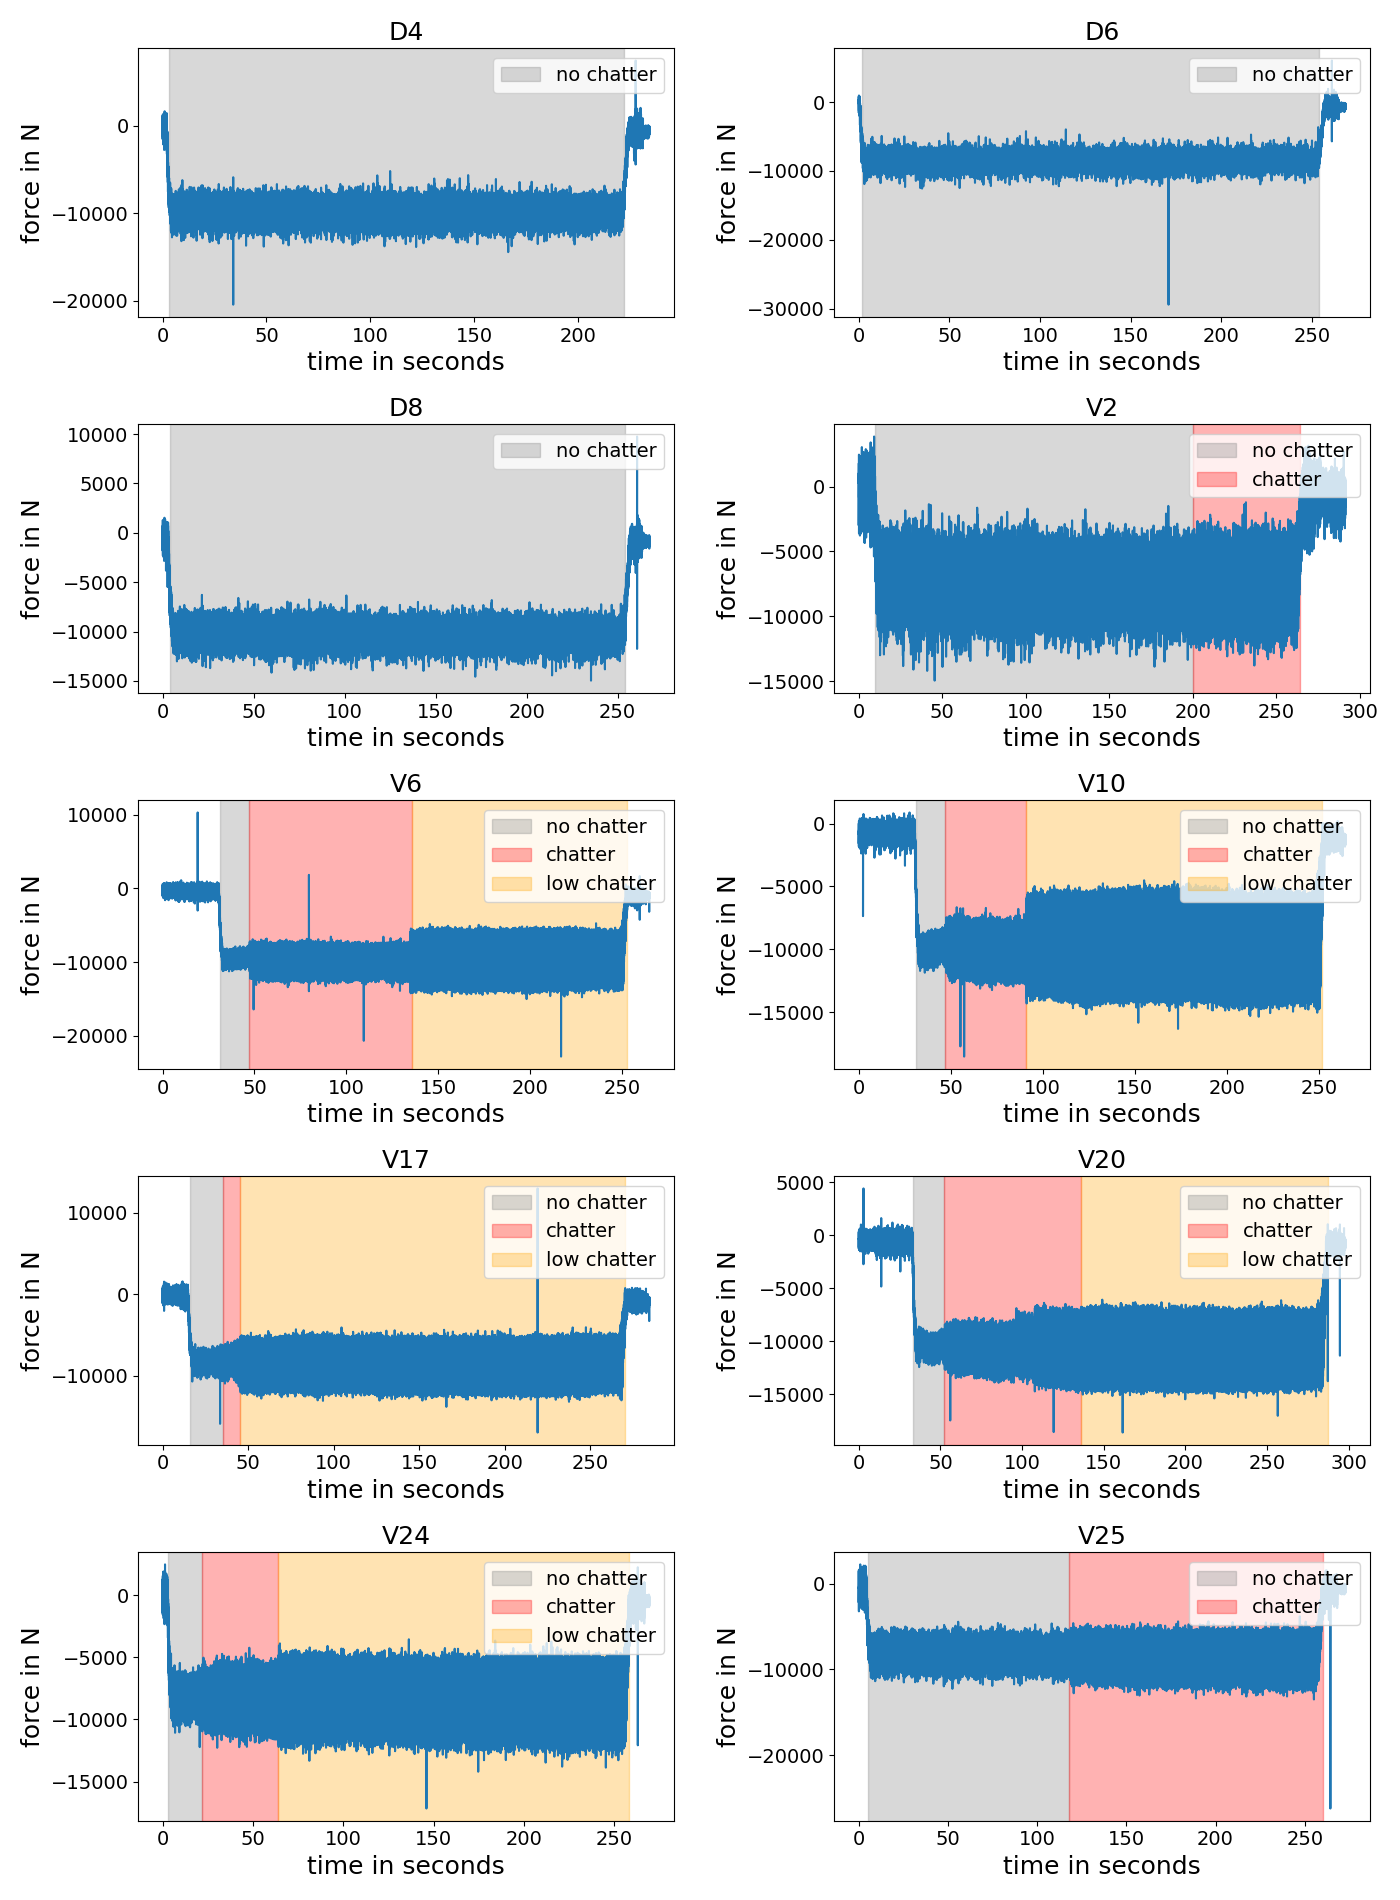
\includegraphics[width=1.1\linewidth]{../plots/all-force.png}
  }
  \caption{Force for all Processes}
  \label{fig:all-force}
\end{figure}

\begin{figure}[p]
  \vspace*{-1cm}
  \makebox[\linewidth]{
    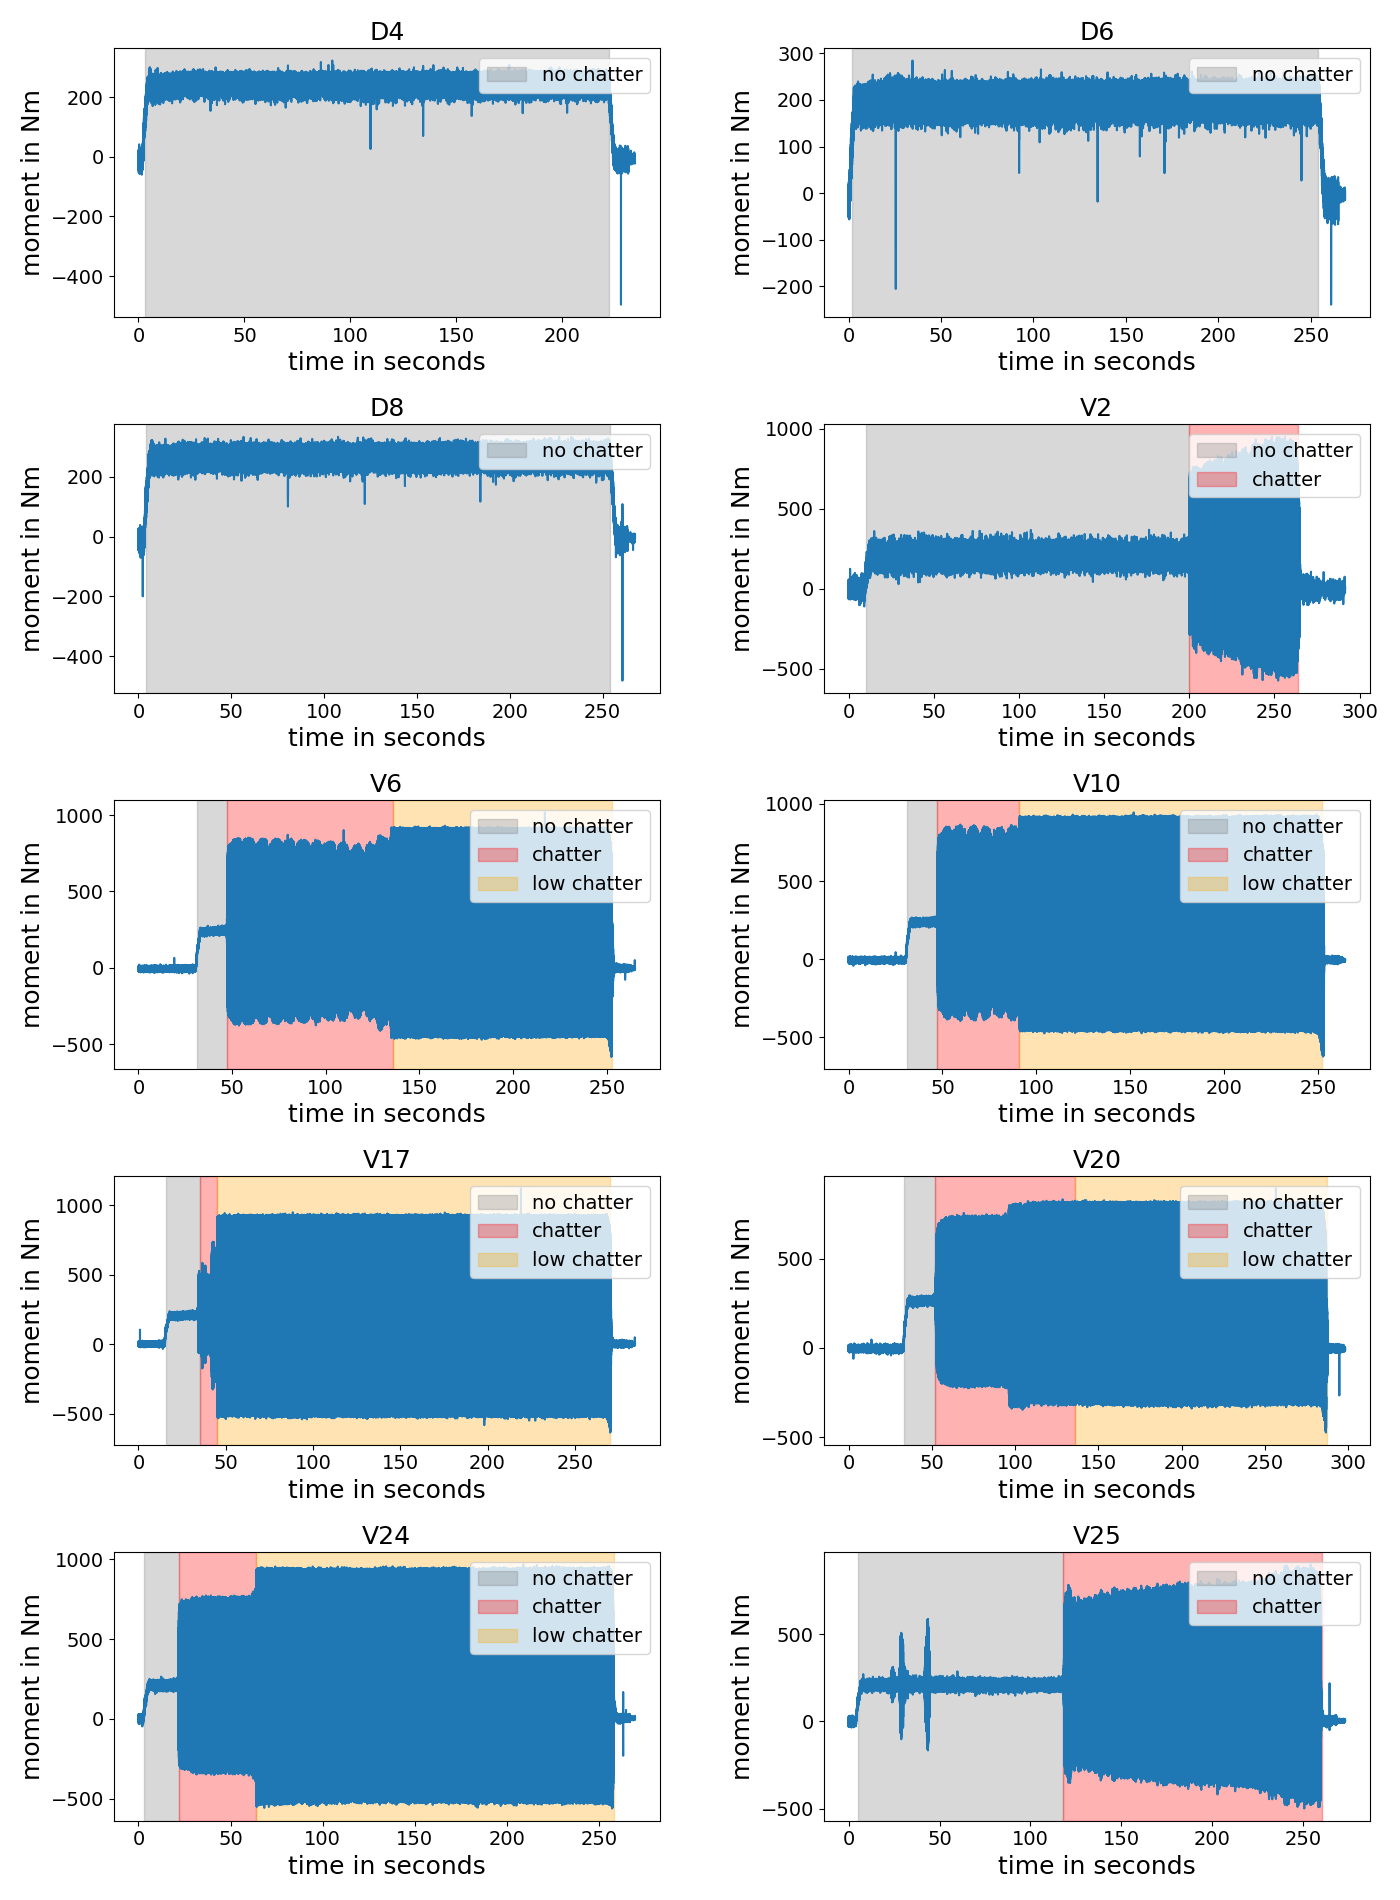
\includegraphics[width=1.1\linewidth]{../plots/all-moment.png}
  }
  \caption{Moment for all Processes}
  \label{fig:all-moment}
\end{figure}

\begin{figure}[p]
  \vspace*{-1cm}
  \makebox[\linewidth]{
    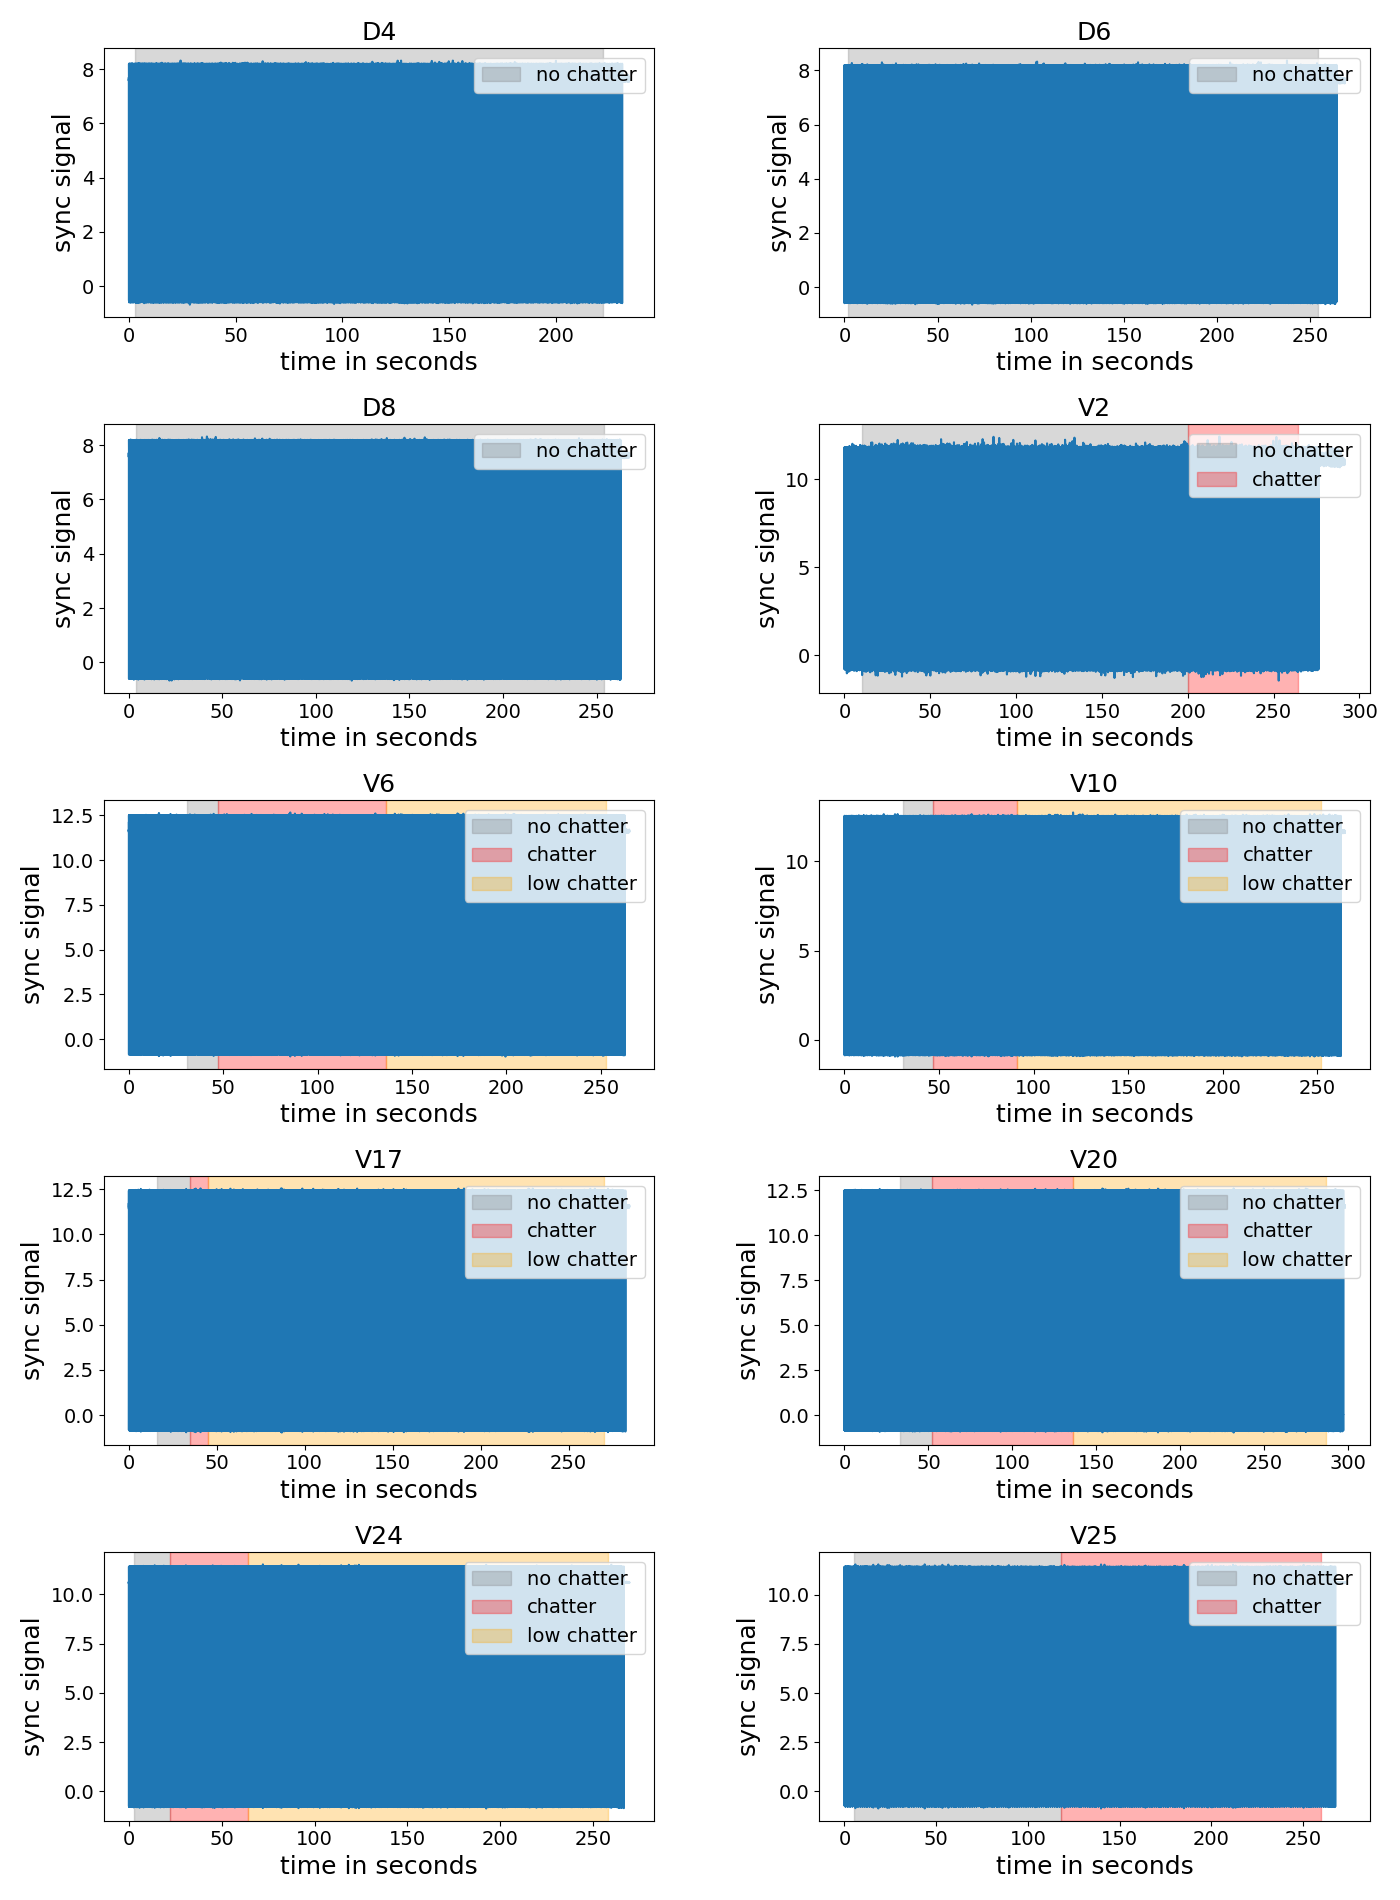
\includegraphics[width=1.1\linewidth]{../plots/all-sync signal.png}
  }
  \caption{Sync Signal for all Processes}
  \label{fig:all-sync}
\end{figure}


\begin{figure}[p]
  \vspace*{-1cm}
  \makebox[\linewidth]{
    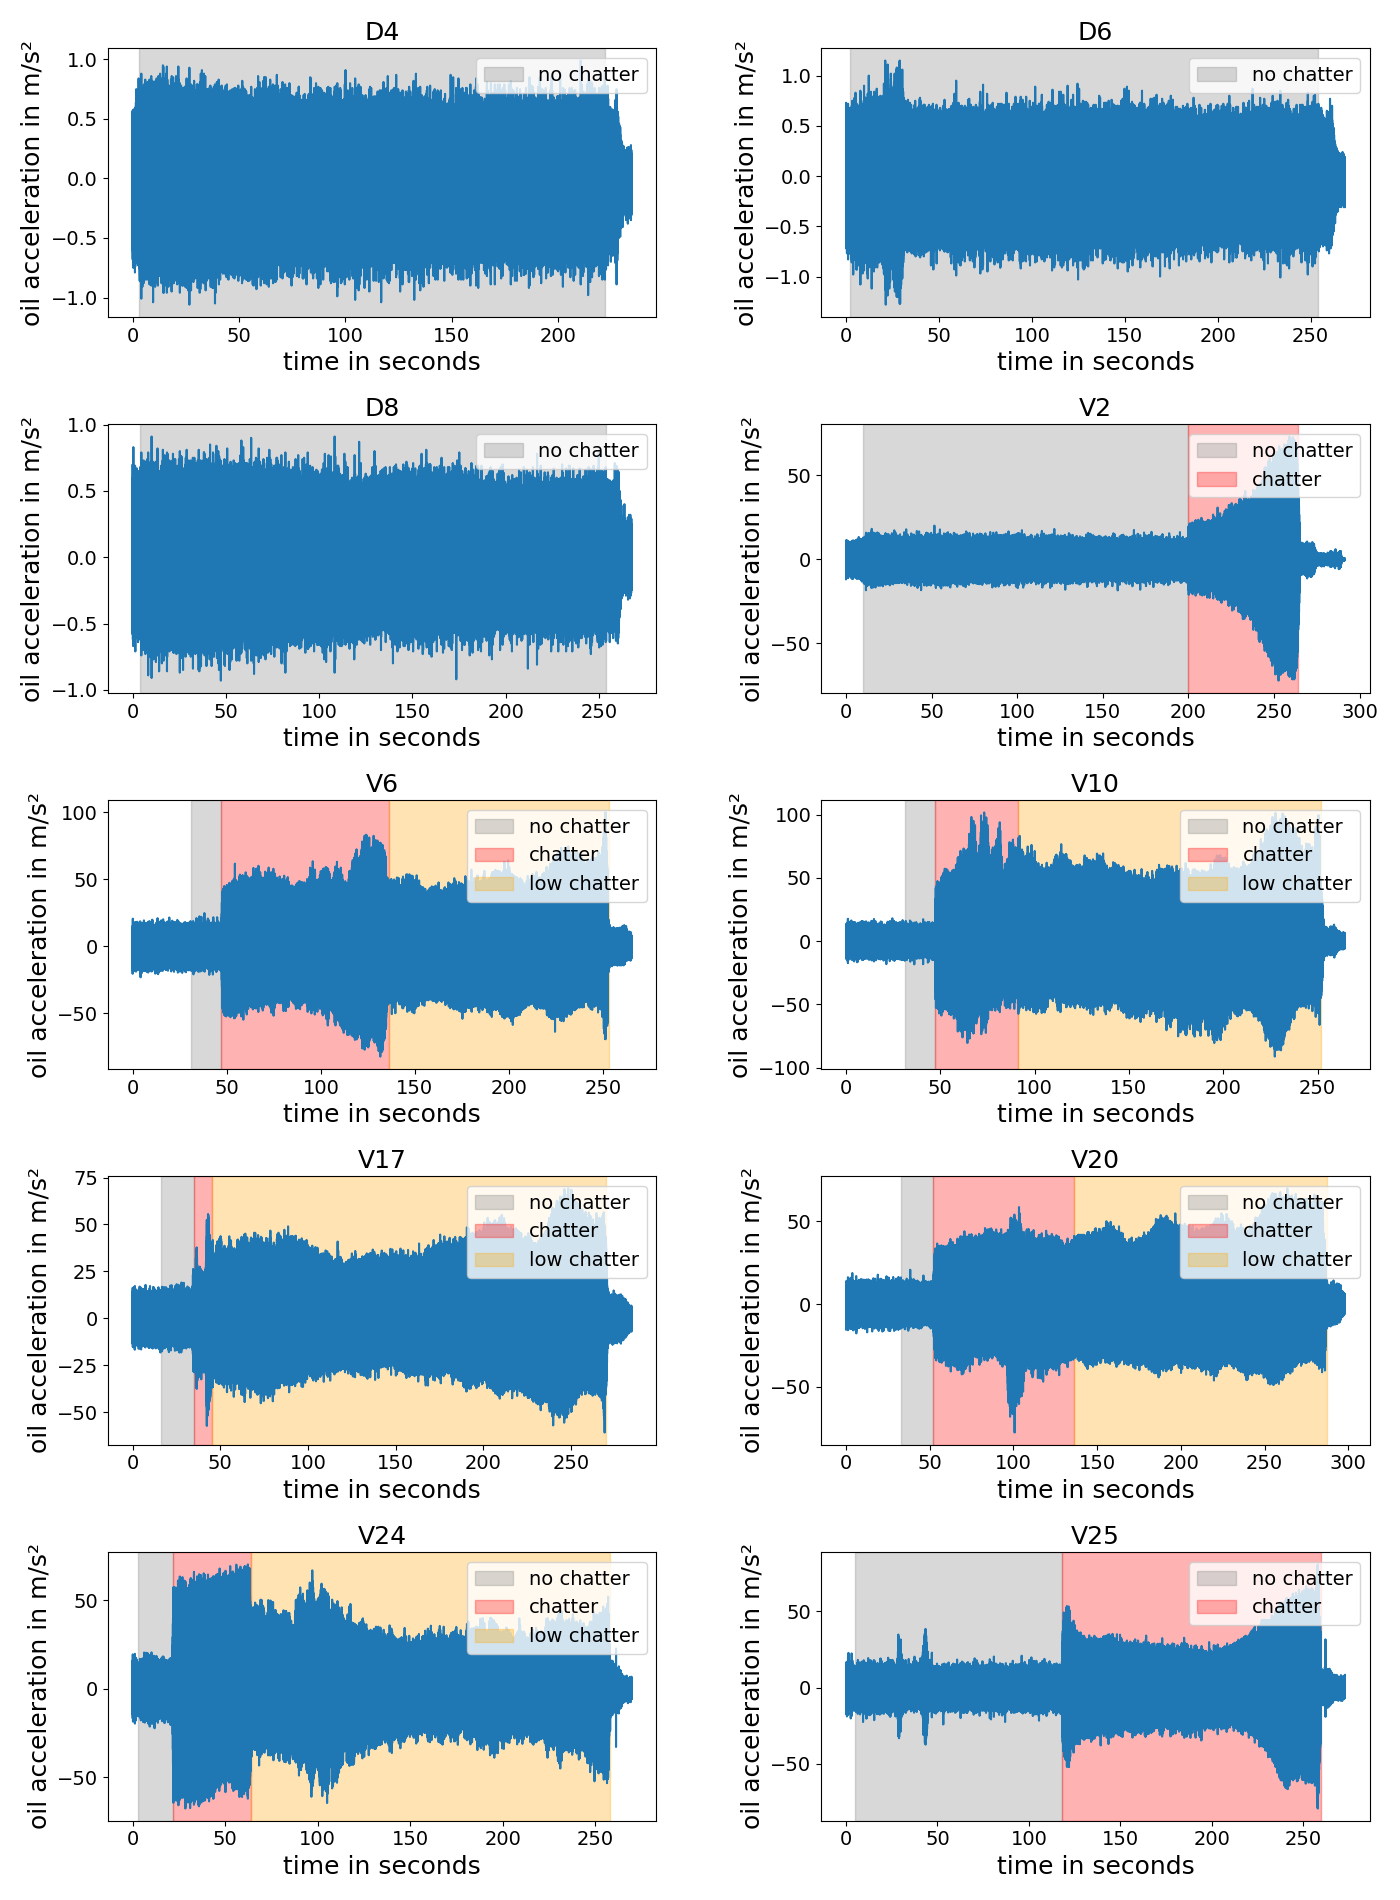
\includegraphics[width=1.1\linewidth]{../plots/all-oil acceleration.png}
  }
  \caption{Oil Acceleration for all Processes}
  \label{fig:all-oil}
\end{figure}

\begin{figure}[p]
  \vspace*{-1cm}
  \makebox[\linewidth]{
    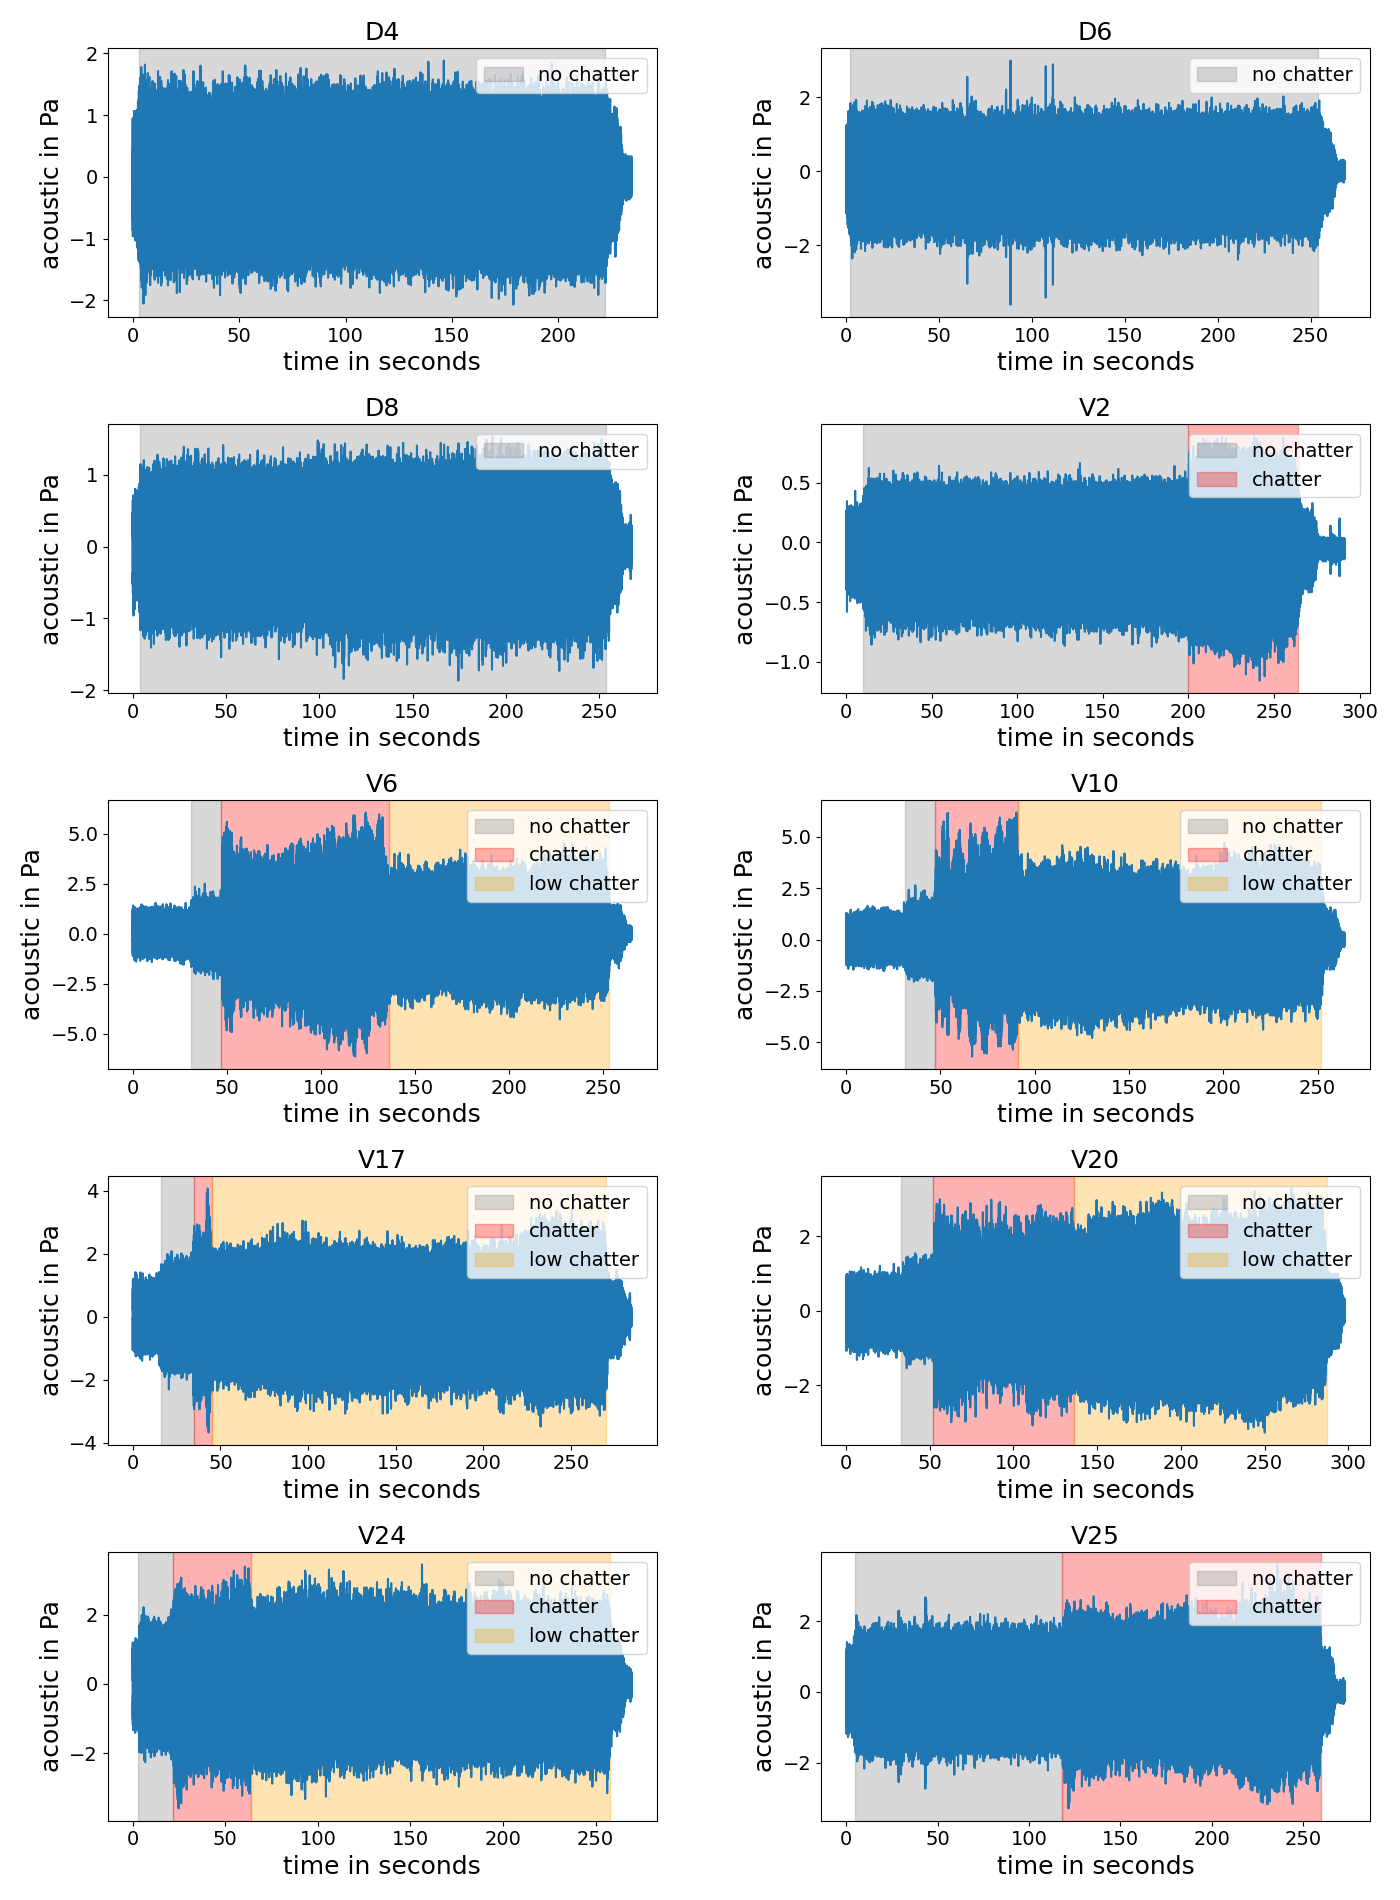
\includegraphics[width=1.1\linewidth]{../plots/all-acoustic.png}
  }
  \caption{Acoustic for all Processes}
  \label{fig:all-acoustic}
\end{figure}


\begin{figure}[p]
  \vspace*{-1cm}
  \makebox[\linewidth]{
    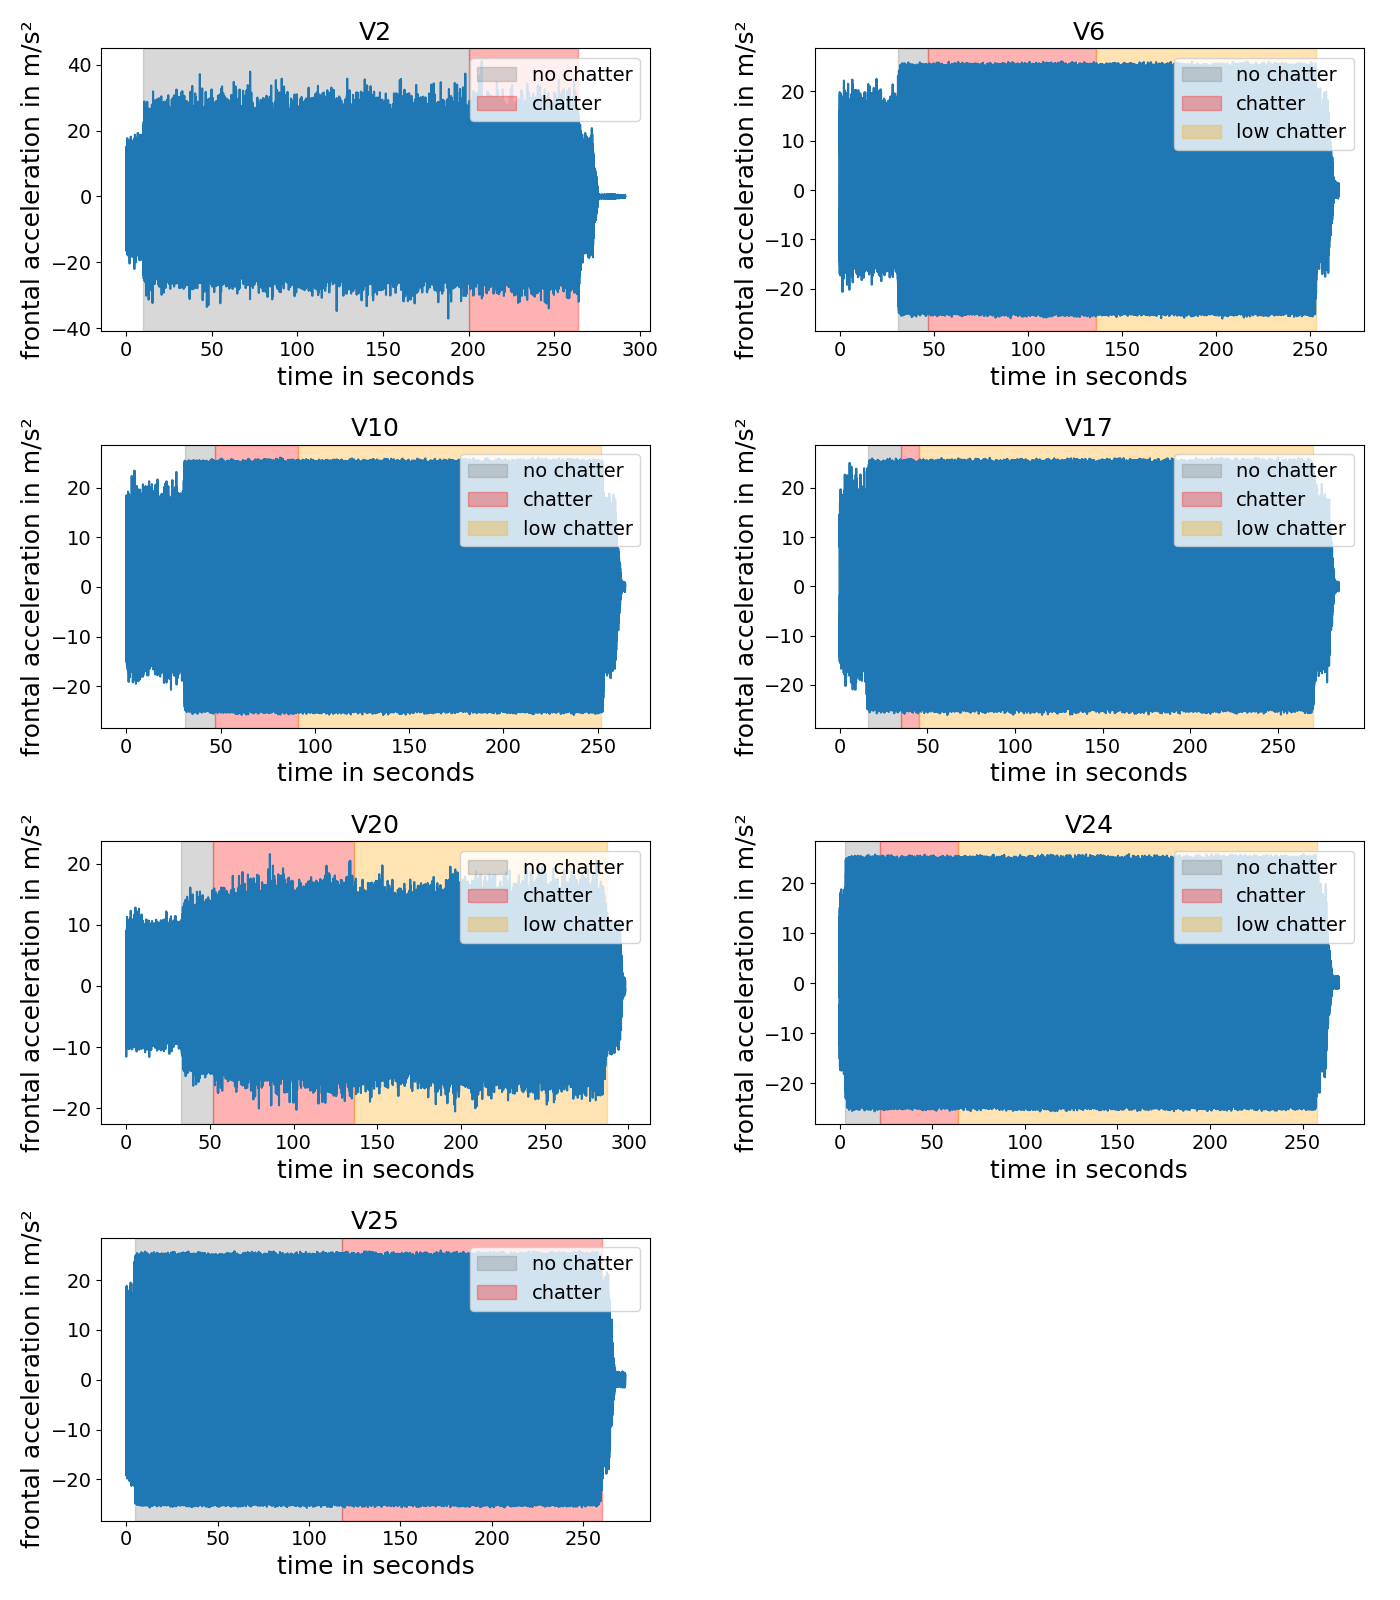
\includegraphics[width=1.1\linewidth]{../plots/all-frontal acceleration m.png}
  }
  \caption{Frontal Acceleration for V-Processes}
  \label{fig:all-frontal}
\end{figure}


\begin{figure}[p]
  \vspace*{-1cm}
  \makebox[\linewidth]{
    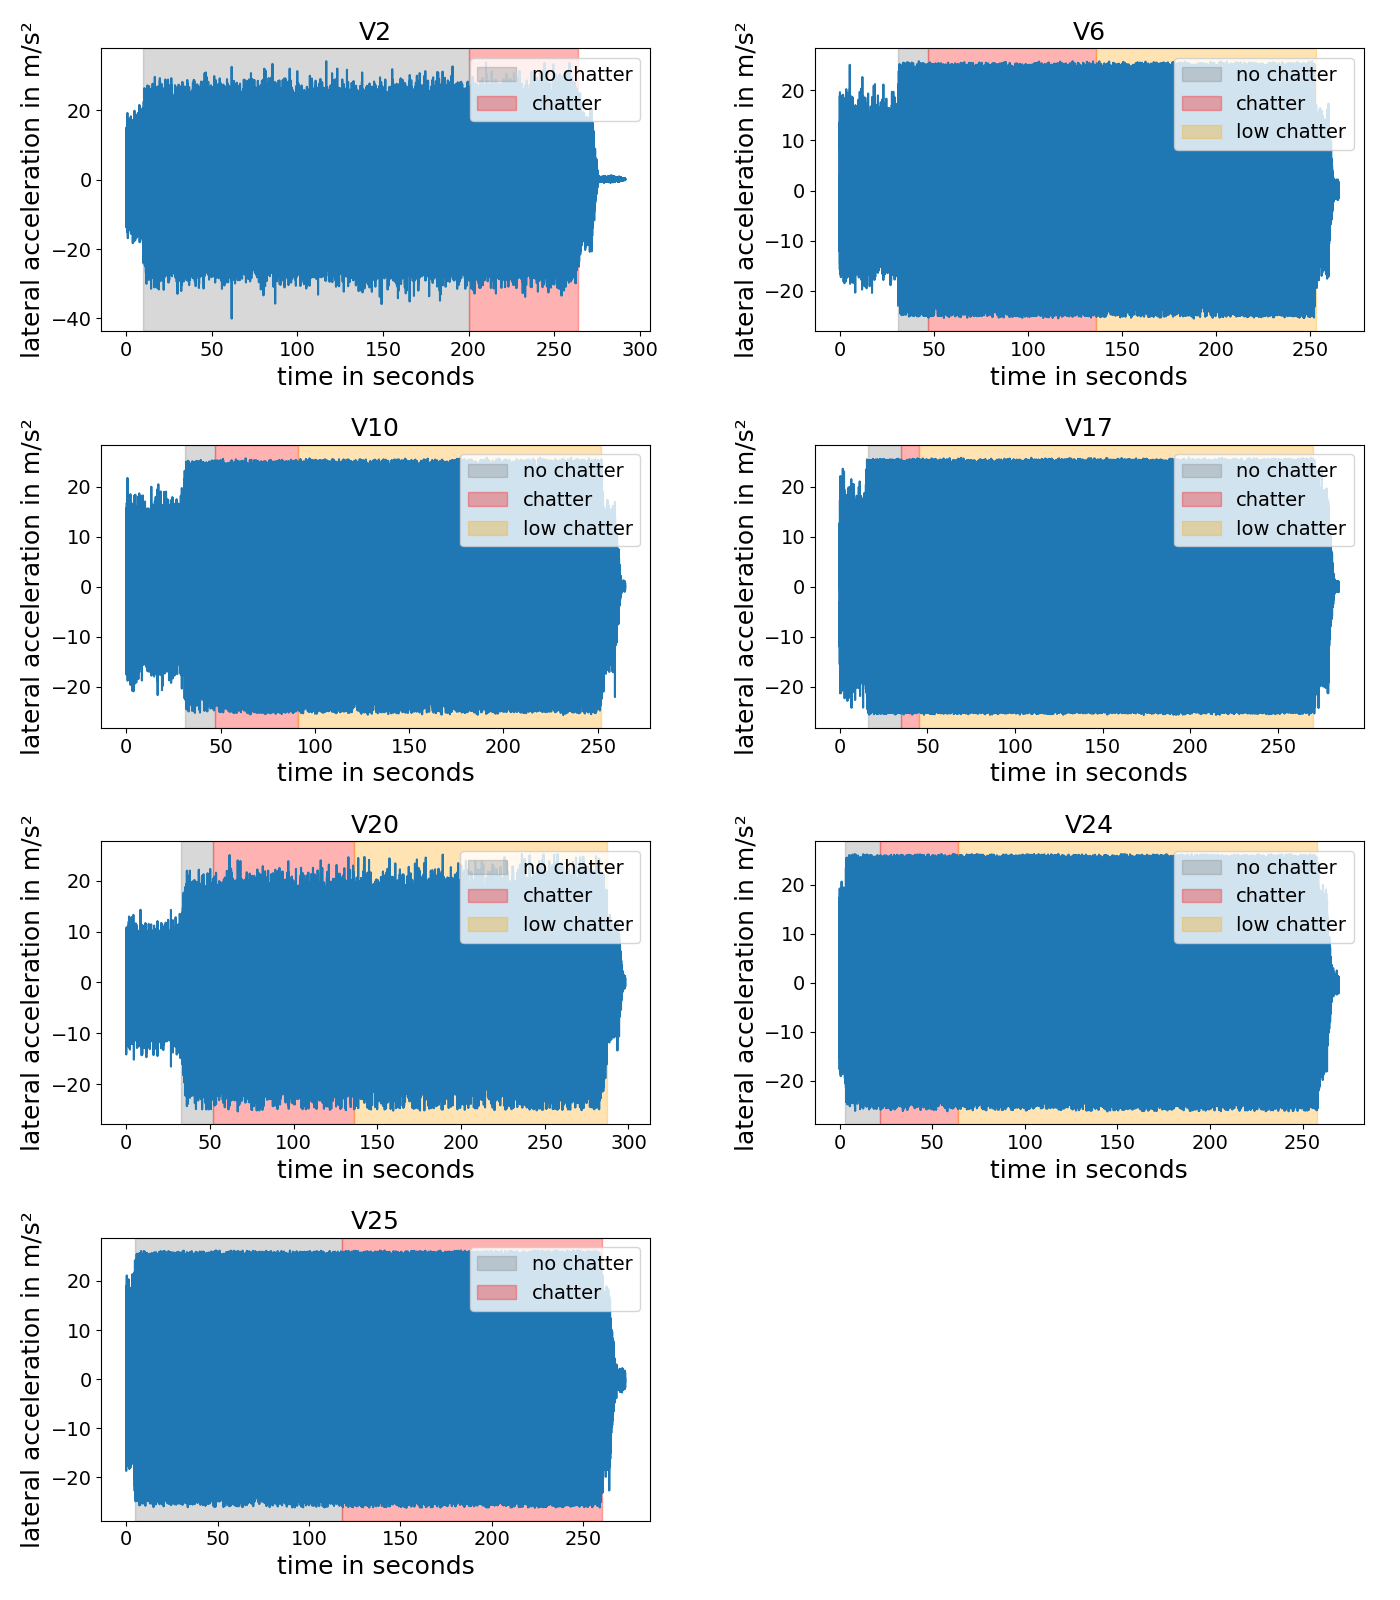
\includegraphics[width=1.1\linewidth]{../plots/all-lateral acceleration m.png}
  }
  \caption{Lateral Acceleration for V-Processes}
  \label{fig:all-lateral}
\end{figure}





\addcontentsline{toc}{subsection}{A \hspace*{0.15cm} Additional figures}
\end{document}
